\documentclass[11pt]{article}

\usepackage[margin = 1in]{geometry}

\usepackage{xcolor}
\definecolor{me}{HTML}{00a31b} %my comments are in green
\newcommand{\me}[1]{{\color{me} #1}}
\definecolor{highlight}{HTML}{ff0000}
\newcommand{\highlight}[1]{{\color{highlight} #1}}
\definecolor{gray}{HTML}{757c87}
\newcommand{\fade}[1]{{\color{gray} #1}}
\usepackage{graphicx}


\usepackage{tikz-feynman}

\usepackage{amsmath}
\usepackage{amsthm}
\usepackage{amsfonts}
\usepackage{amssymb}
\usepackage{slashed}

\newcommand{\defeq}{\ensuremath{:=}}
\newcommand{\corresponds}{\leftrightarrow}
\newcommand{\tr}{\operatorname{tr}}

\newcommand{\grp}[1]{\operatorname{#1}}
\newcommand{\lie}[1]{\mathfrak{#1}}
\newcommand{\vc}[1]{\mathbf{#1}}

\newcommand{\A}{\mathcal{A}}

\newcommand{\ket}[1]{\left | #1 \right \rangle}
\newcommand{\braket}[2]{\left \langle #1 \middle | #2 \right \rangle}

\newcommand{\intd}{\, d}


\begin{document}

%!TeX root = ../main.tex 
\section*{Lecture 2, 18/01/2018}
\subsection*{Introduction}
\me{Throughout there was a lot of historiographic (what word is that for physics?) discussion that I didn't write down.}

Main topic for today is \emph{bosonization.}
We focus on $1+1$ relativistic dimensions although there are generalizations to other cases.
It is an equivalence between (certain classes of) bosonic and fermionic QFTs.

How is this possible, since bosonic theories have boson terms in their Lagrangians and fermionic ones have fermion terms?
Because theories aren't actually determined by their Lagrangians, but by their algebras of operators/correlation functions.

Bosonization is an example of a \emph{duality,} which are good for dealing with nonperturbative phenomena, especially to switch between strong and weak coupling.
Today we just work with free theories, however.

We \emph{will} turn on a self-coupling, and this turns our equivalence of free theories into ``sine-Gordon,'' which has a soliton excitation, \me{whatever that is.}
This is related to massless Schwinger theories (QED with massless fermions in $1+1$ dimensions.)

Apparently one of the people who worked on this was Elliott Lieb \me{who is the same person as the Temperley-Lieb algebra.}
A condensed matter application is to ``Luttinger liquids.''

\subsection*{The theory}
We work a free bosonic scalar field theory of a real-valued field $\phi$ with action
\[
S(\phi) = \int d^D x \left [ \frac{1}{2} (\partial \phi)^2 + V(\phi) \right]
\]
Here the integration measure is Wick rotated to Euclidean signature, even if we are interested in other signatures.
$V(\phi)$ is a potential term that includes masses, self-interactions, etc.
For now $V = 0$.
The partition function is
\[
\mathcal{Z} = \int \mathcal{D} \phi(x) e^{-S(\phi)}
\]
where the phase of the action in the integrand is chosen to make things converge nicely, and is the correct choice. \me{Apparently this was discussed either in the first lecture or last semester?}

The case $D = 2$ is special.
To see why, observe that the correlator
\[
\left \langle \phi(x) \phi(0) \right \rangle = \frac{\Gamma\left(\frac{D-2}{2}\right)}{\left( 4\pi\right)^{D/2}} \left( \frac{1}{x^2} \right)^{\frac{D-2}{2}}
\]
behaves poorly as $D \to 2$.
We will need both a UV and an IR regulator to fix this.

To derive the previous expression:
\begin{align*}
\int \frac{d^D k}{(2\pi)^D} \frac{e^{ikx}}{k^2} &= \int_0^\infty \int \frac{d^D k}{(2\pi)^D} \exp{-sk^2 + ikx}\\
&= \int_0^\infty ds \left( \sqrt{\frac{\pi}{s}} \right)^D \frac{\exp(-x^2/4s)}{(2\pi)^D}\\
&\me{\text{(change variables)}}\\
&= \frac{1}{2^D \pi^{D/2}} \int_0^\infty ds \;s^{D/2-1} \exp(-sx^2/4)\\
\end{align*}
which is equal to the original expression once you write it in terms of the gamma function.

This doesn't work for $D=2$.
To deal with that case we introduce an IR mass regulator $m_0 \ne 0$.
We also change the theory by making it $\phi$-periodic, i.e.~having $\phi$ take values in a circle with radius $R$.
This means that $\phi = \phi+ 2\pi$ and the action becomes
\[
S(\phi) = \frac{1}{g^2}\int d^2 x \left[ \frac{1}{2}(\partial \phi)^2 + \frac{1}{2} m_0 \phi^2 \right]
\]
where the ``coupling constant'' $g = R$ is the radius of the circle.
(It's still called a coupling constant even though it's not actually coupling anything.)

Now, the propagator is
\begin{align*}
G(\phi, m_0^2) &= g^2 \int \frac{d^2 k}{(2\pi)^2} \frac{e^{ikx}}{k^2 + m_0^2}\\
&\approx g^2\left( - \frac{1}{2\pi} \log m_0 + \text{const.} + \mathcal{O}(m_0|x|) \right)
\end{align*}
where $\approx$ means it's an asymptotic expansion.
We get a log divergence in $m_0$.
How do we deal with it?

One consequence: a massless field in $1+1$ dimensions doesn't exist as a quantum object, because of this IR divergence.
This means that there is never any spontaneous symmetry breaking in $1+1$ relativistic dimensions.
This result is the ``Coleman-Mermin-Wagener'' (sometimes also ``Hohenberg'') theorem.
It's really just the converse of Goldstone's Theorem, which says that in a relativistic QFT, if a continuous global internal (i.e.~not spacetime) symmetry is broken, there is a massless mode $\phi$.
In fact, such breaking and modes are in 1-1 correspondence.

If $\phi$ doesn't exist, how is this an interesting theory?
Well, we don't care about the Lagrangian, just the observables.
Even though correlators like $\langle \phi \phi \rangle$ are not well-defined, we still have things like
\begin{itemize}
    \item $\partial_\mu \phi$ and $\epsilon^{\mu \nu} \partial_\nu \phi$, which have to do with the conserved current of the $U(1)$ symmetry
    \item $V_\pm = e^{\pm i \phi}$, so-called ``vertex operators''
\end{itemize}
In particular, we can compute
\[
\left \langle V_+(x_1) \cdots V_=(x_n) V_-(y_1) \cdots V_-(y_m) \right \rangle
\]
at least if it exists when $m_0 \to 0$.
In order to do this we'll need to introduce a UV regulator $\Lambda$ and a corresponding renormalization group scale $\mu$.

For now, focus on the simple case $\langle V_+(x_1) V_-(x_2) \rangle$.
\me{I don't quite follow the details of the next calculation.}
This is a special case of
\[
\left \langle \exp \left( i \int d^2x\; J(x) \phi(x) \right) \right \rangle
\]
for some sourcelike term $J(x)$.
In this case it's $\delta^2(x_1) - \delta^2(x_2)$, so this can be rewritten using the propagator $G$ as
\[
\exp\left( -\frac{1}{2} \int d^2x d^2y\; J(x) G(x,y) J(x \me{\text{ or $y$?}})\right)
\]
where $J(x) = \delta(x_1) - \delta(x_2)$.

In this case this gives
\[
\langle V_+(x_1) V_-(x_2) = \exp\left( -\frac{1}{2} \cdot 2 G(0,m_0^2) + \frac{1}{2} \cdot 2 G(x_1 - x_2,m_0^2)\right)
\]
The first term is a problem on its face, because we'd get a UV divergence as $x \to 0$ in $\log m_0|x|$.
To fix this, we introduce a lattice spacing $a = 1/\Lambda$, which replaces the zero.

Only keeping the logarithmic terms, we then have
\begin{align*}
    \langle V_+(x_1) V_-(x_2) &= \exp \left( \frac{g^2}{2\pi} \left[ \log(m_0/\Lambda) - \log(m_0|x_1 - x_2|) \right]\right)\\
    &= \left( \frac{1}{|x_1 - x_2| \Lambda} \right)^{g^2/2\pi}
\end{align*}
The naive (``engineering'') scaling dimensions of of $\phi$ and $e^{i \alpha \phi}$ (for $\alpha \in \mathbb Z$) are both zero, which would cause problems.
Here quantum fluctuations save us by changing the scaling dimension to $g^2 /4\pi$.
This is an ``anomalous dimension $\gamma$.''

Now to deal with the UV cutoff.
Really the $V_\pm$ are the bare operators, which need to be renormalized.
We rewrite
\[
\left( \frac{1}{|x_1 - x_2| \Lambda} \right)^{g^2/2\pi} = \left( \frac{1}{\mu|x_1 - x_2| } \right)^{g^2/2\pi} \left( \frac{\mu}{\Lambda} \right)^{g^2/2\pi}.
\]
which helps because we can now define (notation used for historical reasons) $\sqrt{Z} V_{\pm}^R = V_\pm$, where
\[
\sqrt{Z} = \left( \frac{\mu}{\Lambda} \right)^{g^2/4\pi}.
\]
Now
\begin{align*}
\langle V^R_+ V^R_- \rangle = \left( \frac{1}{\mu |x_1 - x_2|} \right)^{g^2/2\pi}
\end{align*}
with $[V_\pm^R] = g^2 /4\pi \ne 0$.
We can now compare this to the free Dirac theory.


%!TeX root = ../main.tex 
\section*{Lecture 3, 23/01/2018}
Today we continue with the bosonic theory from last time and compute the correlator
\[
G^{(n,m)}_{\text{bare}} \defeq \left \langle V_+(x_1) \cdots V_+(x_n) V_-(y_1)\cdots V_-(y_m) \right \rangle
\]
As before we use a Gaussian with source a difference of $\delta$-functions:
\[
J = \sum_i \delta(x_i) - \sum_j \delta(y_j)
\]
In $J^2$ there are $n$-self contractions of $\delta(x_i)^2$, $m$ for the $y_j$, $n(n-1)$ of $x_i$ with a different $x_{i'}$, $m(m-1)$ for the $y_j$, and $nm$ $xy$ terms.
We get an overall factor
\[
G_{\text{bare}}^{(n,m)} \sim m_0^{n+m+n(n-1) + m(m-1) - 2nm} = m_0^{(n-m)^2}
\]
Thus in the $m_0 \to 0$ limit the correlators are zero unless $n=m$:
\[
G^{(n,m)} = m_0^{\frac{g^2}{2 \pi} (n-m)} \left( \frac{1}{\Lambda}\right)^{\frac{g^2}{4\pi} (n+m)} \left( \frac{\prod_{i\ne i'} |x_i - x_{i'}| \prod_{j \ne j'} |y_j - y_{j'}|}{\prod_{i,j} |x_i - y_j|}\right)^{\frac{g^2}{2\pi}}
\]

The nonzero case is a clue towards a symmetry.
In this case it's that the massless field $\phi$ has a global $U(1)$ symmetry given by $\phi \mapsto \phi + \text{const}$.
Furthermore, the renormalized propagator is
\[
G^{(n,n)}_{(R)} = \left( \frac{1}{\Lambda}\right)^{\frac{g^2}{2\pi} n} \left( \frac{\prod_{i\ne i'} \mu |x_i - x_{i'}|  \prod_{j \ne j'} \mu |y_j - y_{j'}|}{\prod_{i,j} \mu|x_i - y_j|}\right)^{\frac{g^2}{2\pi}}
\]
This is secretly a fermion theory.

The RG equation for this theory (a simple version of the Callan Symanzik equation) is
\begin{align*}
0 &= \mu \frac{\partial}{\partial \mu} \\
&= Z^n \left( \mu \frac{\partial}{\partial \mu}^{2n} + 2n \mu \frac{\partial \log \sqrt Z}{\partial \mu} \right) \left \langle V_+^{(R)} \cdots V_-^{(R)} \right \rangle\\
&= \left( \mu \frac{\partial}{\partial\mu} + 2n \frac{g^2}{4\pi}\right) G^{(n,n)}_{(R)}
\end{align*}
Compare to the general formula for dependence on the RG scale:
\[
\left( \mu \frac{\partial}{\partial \mu} + \beta(g) \frac{\partial}{\partial g} + n \gamma_+(g) + n \gamma_-(g) \right) G_{(R)}(x;\mu;g).
\]
Here $\mu$ is the scale, $g$ is a coupling constant, and $\gamma_\pm$ are the ``anomalous quantum dimension(s).''
In our case the beta function vanishes, so we get exact CFTs everywhere \me{in R(?)}
More generally, CFTs with central charge $c = 1$ have been completely classified; we will return to this later.

\subsection*{Fermionic theory}
We now work with free Fermions in $\mathbb{R}^{1+1}$, flat Lorentz spacetime Wick rotated to Euclidean signature.
To \emph{really} check equivalence we should examine other topologies, but we won't bother.
Maybe in a string theory course.

Below $\psi$ is a Dirac fermion.\footnote{We could use a pair of Majorana fermions, since those are equivalent in genus zero, but they aren't in other cases so we won't.}
We do the usual thing with $\psi = \begin{bmatrix} \psi_+ \\ \psi_- \end{bmatrix}$ and write the action as
\[
S(\psi, \bar \psi) = \int dz d\bar z \; \left( \bar \psi_+ \partial_{\bar z} \psi_+ + \bar \psi_- \partial_z \psi_-\right)
\]
This has a classical $U(1) \times U(1)$ symmetry parametrized by $\theta, \theta_5$:
\begin{align*}
\psi &\mapsto e^{i \theta +i \theta_5 \gamma_5} \psi\\
\psi &\mapsto e^{-i \theta +i \theta_5 \gamma_5} \psi
\end{align*}
where $\gamma_5$ is the \emph{third} gamma matrix and is called that in analogy with dimension 4.
The currents are
\begin{align*}
J_\mu &= \bar \psi \gamma_\mu \psi\\
J_\mu^5 &= i \bar \psi \gamma_5 \gamma_\mu \psi
\end{align*}
Since (depending on your $\gamma$ matrix conventions) $i \gamma_5 \gamma_\mu = - \epsilon_{\mu \nu} \gamma^\nu$ the currents are related to one another.

Now the propagators are 
\begin{align*}
\Delta^+ &= \left \langle \bar \psi _+(z,\bar z) \psi_+(0)\right \rangle = - \frac{1}{2\pi z}\\
\Delta^- &= \left \langle \bar \psi _-(z,\bar z) \psi_-(0)\right \rangle = - \frac{1}{2\pi \bar z}.
\end{align*}
Then (have to have the same number of $\psi$ and $\bar \psi$ terms)
\[
\left \langle \prod_{i=1}^n \bar \psi_+(z_i) \psi_+(z_i') = \left ( -\frac{1}{2\pi} \right)^n \det \left [ \frac{1}{z_i - z_j'}\right]_{ij} \right \rangle
\]
and similarly for $-$ but with $\bar z_i$ on the right-hand side.
\me{Here we wrote out expressions for $J_1$ and $J_2$ but I'm not sure why.}

Now, if we write $\sigma_+ = \bar \psi_- \psi_+$ and $\sigma_- = \bar \psi_+ \psi_-$, we find that their correlators are the same as in the bosonic theory.
Specifically, define $\varphi$ to be the same as $\phi$ but $R$-periodic \me{(instead of $2\pi$-periodic.)}
Then the map
\[
2 \pi \sigma_\pm \mapsto \mu \left[ e^{\pm i \sqrt{4\pi} \varphi} \right]_{(R)}
\]
is an equivalence
\begin{align*}
\bar \psi \slashed \partial \psi &\leftrightarrow \frac{1}{2} (\partial_\mu \varphi)^2\\
\bar \psi \gamma^\mu \psi &\leftrightarrow \frac{\varepsilon^{\mu\nu}}{\sqrt \pi} \partial_\nu \varphi \equiv j^\mu \sim \epsilon^{\mu \nu} \mathcal{J}_\nu
\end{align*}
\me{not sure what the stuff on the end is about.}
This is an ``electric-magnetic duality'' and can be compared to $T$-duality in a string theory context.

We can now start filling in a diagram of theories with ``one degree of freedom,'' which rigorously means CFTs with central charge $1$ (when parametrized correctly.)
Here's a partial chart, where $\#$ is some dimensionful constant \me{like string length.}
\begin{center}
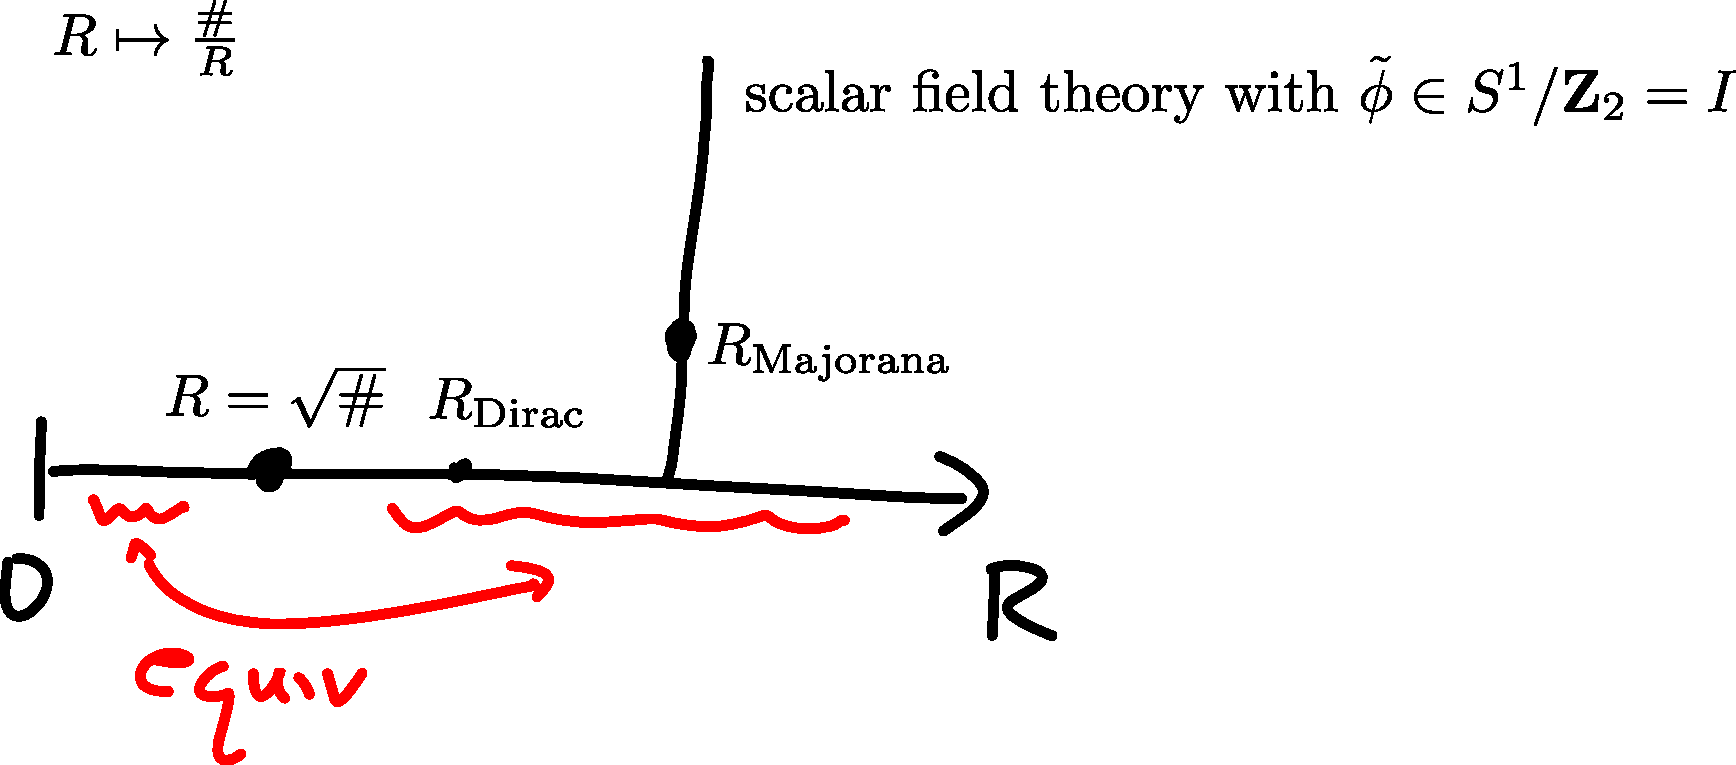
\includegraphics[width = 7in]{fig/lecture3CFTchart.pdf}
\end{center}






%!TeX root = ../main.tex 
\section*{Lecture 4, 25/01/2018}
\me{I missed the first 20 minutes but I think it was just review of last time.}

We previously computed
\begin{align*}
\left \langle \prod_1^n \sigma_+(x_i) \sigma_-(y_j) \right \rangle &= (-1)^n \left \langle \prod_1^n \bar \psi_+(y_i) \psi_+(x_i) \right \rangle\\
&= \left ( \frac{1}{2 \pi} \right)^{2n} \left [ \frac{ \prod_{i < j} |x_i - x_j|^2 |y_i - y_j|^2 }{ \prod_{i,j} |x_i - y_j|^2 } \right ]^{g^2/4 \pi}.
\end{align*}
To get this to match up, we need $g^2/4 \pi = 1$, so now we just set $g = \sqrt{4\pi}$.
The correlator above is supposed to be equal to
\begin{align*}
\left( \frac{1}{2 \pi}\right)^{2n} \left \langle \prod_{i = 1}^n \mu^2 V_+^{(R)}(x_i) V_-^{(R)}(y_i) \right \rangle,
\end{align*}
so we posit that
\begin{align*}
\sigma_\pm &= \mu V_\pm^{(R)}\\
V_\pm^{(R)} &= \left( \frac{\Lambda}{\mu} \right)^{g^2/4 \pi} V_\pm
\end{align*}
so that
\begin{align*}
\bar \psi_- \psi_+ &= \frac{\Lambda}{2 \pi} e^{i \phi}\\
\bar \psi_+ \psi_- &= \frac{\Lambda}{2 \pi} e^{-i \phi}
\end{align*}

Note that when defining $\varphi = \phi/g$ (choosing a canonical length scale) so that $\varphi = \varphi + 2 \pi$) we instead get $\bar \psi_- \psi_+ = e^{i \sqrt{4\pi} \varphi}$, etc.
This convention is in some (most?) literature.
More generally, the correspondence is
\begin{align*}
\bar \psi \slashed \partial \psi &\corresponds \frac{1}{2} (\partial_\mu \varphi)^2\\
j^\mu \defeq \bar \psi \gamma^\mu \psi &\corresponds \frac{\varepsilon^{\mu \nu}}{\sqrt \pi} \partial_\nu \varphi\\
\bar \psi \psi &\corresponds \Lambda \cos(\sqrt{4 \pi} \varphi)\\
\bar \psi \gamma^0 \gamma^1 \psi &\corresponds \Lambda \sin(\sqrt{4 \pi} \varphi)
\end{align*}
\me{The last was written using $\gamma_* \defeq \gamma^0 \gamma^1$ but this notation was not used again.}

\subsection*{Application one of bosonization}
Often we want to add a self-interaction density $\rho(x) V(x,y) \rho(y)$ to a theory.
This density $\rho$ is really $j^0$.
We now get a term $j^0 V j^0$ that is quartic in $\psi$, but bosonization lets you turn this in a term like $(\partial_0 \varphi)^2$, which is quadratic and therefore can be computed using a Gaussian.

\subsection*{Application two of bosonization}
Consider a simple $(1+1)$-dimensional condensed matter system, say a lattice model with operators $\psi(n), \psi^\dagger(n)$ on each vertex, with $\{ \psi^\dagger(n), \psi(m) \} = \delta_{m+n}$. 
(It's not immediately clear that this is relevant, since it's a non-relativistic system, but we'll get there.)
We use a Hamiltonian of the form
\[
H = - \sum_{n \in \mathbb Z} \psi^\dagger (n) \psi(n+1) + \text{h.c.}
\]
The Fourier transform of this is
\[
H = - \int_{-\pi}^\pi \frac{dk}{2 \pi} (\cos k) \psi^\dagger \psi
\]
where these $\psi$s are actually the momentum-space versions.

The ground state is a Fermi sea.
It looks like a graph of $- \cos$ on $[-\pi, \pi]$, and the 1-d excitations live near the zeros, at $\pm \pi/2$.
Zooming in it's a line with slope $c$, and the excitations move with $\omega = \pm ck$, where $k$ is the difference.
These are like free Dirac fermions.

In \emph{more} dimensions this doesn't quite work: you in general get a $(d-1)$-sphere of fermions, and for $d > 1$ this has infinitely many points, which is hard to deal with.

\subsection*{Massless Schwinger model}
Here the action is (expanding out the gauge derivative $\slashed D$) is
\[
S = \int d^2 x \left[ \bar \psi \slashed \partial \psi + A_\mu j^\mu - \frac{1}{4 e^2} F_{\mu \nu}F^{\mu \nu}\right],
\]
where we put the electric charge $e$ with the $F^{\mu \nu}$ term to match the usual conventions for a Yang-Mills theory.
This theory is potentially complicated because of the interaction terms: you get \emph{lots} of Feynman diagrams.
However there are simplification.

In two dimensions, the $\beta$ function is dimensionful, so the theory is superrenormalizable, i.e.~free in the UV limit.
Another interesting feature is that there are zero polarizations (compare $3-1 = 2$ in reality), bt least classically.
When we quantize we'll get new things and the theory won't be trivial.

To solve the theory we use the correspondence $\psi \bar \psi \corresponds \varphi$ \me{the $\psi$ term looks wrong here} to change the action to
\[
S = \int d^2 x \left [ \frac{1}{2} (\partial_\mu \varphi)^2 + \frac{\partial_\mu \varphi}{\sqrt \pi} \partial^\mu f + \frac{1}{2e^2} \partial^2 f \partial^2 f\right],
\]
where we have written $A_\mu = \partial_\mu \alpha + \varepsilon_{\mu \nu} \partial^\mu f$ and (locally) gauge transformed $\alpha = 0$.
We work in Minkowski signature, so that $\varepsilon_{01} = 1$, $\eta_{00} = 1$, $\eta_{11} = -1$, $\varepsilon^{01} = -1$, and $\varepsilon_{\mu \nu} \varepsilon^{\nu \sigma} = \delta_\mu^{\phantom{\mu} \sigma}$.

Notice that we have turned a cubic self-interaction into a quadratic term!
This is a \emph{free} bosonic theory.

Actually, we should also integrate by parts to change the middle term to $- \frac{\varphi}{\sqrt \pi} \partial^2 f$, so that
\begin{align*}
S &= \int d^2 x \left[ - \frac{1}{2 \pi} \partial_\mu f \partial^\mu f + \frac{1}{2e^2} \partial^2 f \partial^2 f\right]\\
&= \int d^2 x \left[ \frac{1}{2 \pi} A_\mu A^\mu + \frac{1}{2e^2} A_\mu \partial^2 A^\mu\right]
\end{align*}
\me{I don't really get what's happening here.}

The result is a theory of a propagating scalar with
\[
\left \langle A_\mu A_\nu \right \rangle = \left( \eta_{\mu \nu} - \frac{p_\mu p_\nu}{p^2} \right) \frac{1}{p^2 - e^2/\pi}
\]
with corresponding dispersion relation $\omega^2 = k^2 + e^2/\pi$.
The two-point function has no cuts, just poles, so we get \emph{confinement:} there are no asymptotic states with charge.

``Spontaneous breaking of chiral symmetry'' \me{is a phrase stated at the end of class.
It may be related to
\[
\langle \sigma_\pm \rangle = \frac{\Lambda}{2 \pi} \langle e^{\pm i \theta} \rangle
\]
and a new scalar field $\theta$.
Apparently in the above the $\Lambda$s cancel.}

%!TeX root = ../main.tex 
\section*{Lecture 5, 30/01/2018}
We discussed the bosonization correspondence from before, and returned to the chart of relativistic CFTs with ``one degree of freedom'' in $1+1$ dimensions.
Main new comment was that it follows an ADE classification: the two axes are the A and D and the E refers to the three isolated theories.
The reason for this has to do wtih classifying the discrete subgroups of $\operatorname{SU}(2)$.

\subsection*{Thirring and sine-Gordon}
``Sine-Gordon'' is a pun on ``Klein-Gordon'' since there's a (co)sine in it.
The action is
\[
S_{\text{SG}} = \int d^2x \left [ \frac{1}{2} \partial_\mu \varphi \partial^\mu \varphi + \frac{m^4}{\lambda} \cos\left ( \frac{\sqrt \lambda}{m} \varphi\right ) \right ]
\]
Here $m$ is the mass and $\lambda$ is the self-coupling.
The $m^4$ is the right thing to do for a theory in $1+1$ dimensions.
Sometimes there's a $1$ subtracted from the cosine to make the theory have $\varphi = 0$ give zero energy, but absolute energy levels don't matter so we drop it.
This theory is integrable both clasically and on a quantum level.

The equation of motion is
\[
\partial^\mu \partial_\mu \varphi + \frac{m^2}{\lambda} \sin \left(\frac{\sqrt \lambda }{m} \varphi \right)
\]
which has infinitely many zero-energy solutions because of the periodicity.
We could do perturbative expansion around each one and they wouldn't interact, because it's not possible to jump between wells like that in infinite space.
\me{There was a comment about that being true clasically but not when we quantize but I'm not sure what the actual statement is.}

Instead we quantize a \emph{soliton}, which for our purposes means a thing that doesn't dissipate, usually associated to a conserved quantity.
Once we have one we can boost it to any velocity \me{and quantize around these.}

Define $\bar x = mx$, $\bar t = mt$, $\bar \varphi = \frac{\sqrt \lambda}{m} \varphi$.
We have symmetries $\bar \varphi \mapsto - \bar \varphi$, $\bar \varphi \mapsto \varphi + 2\pi$.
If $\bar \varphi (- \infty ) = 2 \pi N_1$ and $\bar \varphi(\infty) = 2 \pi N_2$, then we get a ``topological charge''
\[
Q = N_1 - N_2 = \frac{1}{2 \pi} \int d \bar x \partial_{\bar x} \bar \varphi \sim \int d \bar x j^0
\]
Note that $\varphi \mapsto \varphi + c$ is \emph{not} a symmetry of the theory.

For $Q = \pm 1$ we get soultions
\[
\bar \phi (x) = \pm 4 \operatorname{atan} e^{-\bar x - \bar x_0}
\]
which we call solitons and antisolitions.
\me{(Many of the formulas here may be wrong.)}
They have scattering
\[
4 \operatorname{atan} \left( \frac{\sinh(u \bar t/ \sqrt{1-u}) }{u \cosh(\bar x \sqrt{1-u^2}) } \right).
\]
\me{Under $u \mapsto iv$??} we get ``breather'' or ``doublet'' solutions
\[
\bar \phi = 4 \operatorname{atan}\left[ \frac{\sin(\pi \bar t/\sqrt{1+v^2})}{v \cosh (\bar x /\sqrt{1+v^2})}\right]
\]
Also, the energy of the classical solution is $8m^3/\lambda$, while the energy of the quantum solution is $8m^3/\lambda + m/\pi + \mathcal{O}(\lambda).$ \me{There was a comment about the importance of that that I missed.}

We return to the original model to bosonize. With $\phi = \frac{\sqrt{\lambda}}{m} \varphi$, we have
\[
S_{\text{SG}} = \frac{m^2}{\lambda} \int \frac{1}{2} (\partial_\mu \phi)^2 + m^2 \cos \phi
\]
The coupling constant $g$ from before is now usually called $\kappa$, with $\kappa^2 = \lambda/m^2$.
The proof \me{of the following (?)} is careful and order-by-order but we don't discuss it.

The Thirring model is
\[
S_T = \int d^2 x \left[\bar \psi (\slashed \partial + m_F) \psi - \frac{1}{2} g J_\mu J^\mu \right].
\]
When bosonizing: the $\slashed \partial$ term becomes $(\partial_\mu \varphi)^2$, the $m_F$ term becomes $\Lambda \cos \varphi$, and the final term gets two $\varepsilon^{\mu \nu}$s, which combine to give an $\eta^{\mu \nu}$, so it becomes $(\partial_\mu \varphi)^2 g / \pi$.
We have thus shown that
\[
1 + \frac{g}{\pi} = \frac{4\pi}{\kappa^2}
\]

Implications:
\begin{itemize}
    \item The fermion mass $m_F$ is zero \me{(?)}
    \item The sine-Gordon theory can be shown to be non-renormalizable, so we've shown that Thirring isn't either, which would have been much harder directly.
    \item The fermion $\psi$ corresponds to the soliton in the sine-Gordon theory.
\end{itemize}

In the next lecture, we will discuss quantization of (non-abelian) Yang-Mills theories.

%!TeX root = ../main.tex 
\section*{Lecture 6, 01/02/2018}
Today we discuss Yang-Mills theories, for now in Minkowski spacetime of $3+1$ dimensions.

In 1954 QED was figured out, which is a theory of a potential $A_\mu$ and fields $\psi$, $\phi$, etc.
It was very succesful, and used an \emph{abelian} $\grp U (1)$ gauge symmetry.
Attempts to generalize this to non-abelian gauge groups were considerably more difficult, and this is what we explain now.

Recall that for a scalar field $\phi(x)$, gauge invariance requires us to promote $\partial_\mu$ to a \emph{covariant derivative}
\[
D_\mu(A) \defeq \partial_\mu - i e A_\mu.
\]
This results in a $U(1)$ invariant theory and automatically includes self-interactions of the gauge field $A_\mu$.

We now promote $\phi$ to a vector $\phi^i$ and the symmetry group to $\grp U(N)$ (or some other compact Lie group $G$.)
Now the transformation $\phi(x) \mapsto U \phi(x)$ is a symmetry of the action
\[
S = \int \partial \bar \phi \partial \phi \pm m^2(\bar \phi \phi) + \frac{\lambda}{\text{numerical constant}} (\bar \phi \phi)^2
\]
This is an invariant ``global'' symmetric because it acts on all of spacetime in the same way.
It could be ``broken,'' which means that the vacuum state is not preserved by the charges ($Q \left | 0 \right \rangle \ne 0$.)
If it isn't, we get an actual symmetry acting on the states.

We now want to ``gauge'' this symmetry by promoting it to a ``local'' symmetry
\[
\phi(x) \mapsto U(x) \phi(x)
\]
For this to work we need a \emph{covariant} derivative.
Observe that
\[
\partial_\mu(U \phi) = U \partial_\mu \phi + (\partial_\mu U) \phi = U(\partial_\mu \phi + (U^{-1} \partial_\mu U)) \phi,
\]
so we postulate
\[
D_\mu \phi^i(x) = \partial_\mu \phi^i - i A_\mu^{ij}(x) \phi^j(x)
\]
where now $A_\mu$ is ``matrix-valued,'' taking values in the adjoint representation of the gauge group $G$, which is to say in its Lie algebra $\lie g$.
Notice that we've absorbed the charge into $A_\mu$, which is more convenient right now, although we'll want it back when we do perturbative calculations.
In this convention, $[A_\mu] = [\partial_\mu] = 1$, which is convenient.

\me{Here there was a brief discussion of Lie theory: $\lie g = T_eG$, the exponential map, the Killing form, etc.
I already knew about this so I didn't write it down, but there was a mention of Zee's book on group theory as a good reference.}
We will only work with compact gauge groups $G$ for now, although we might allow non-compact ones later when we talk about Chern-Simons theories.
Note that physicists frequently forget about $\lie g$ and just call everything $G$.
We work in a basis $T^a$ of $\lie g$ that diagonalizes the Killing form.

Now, under the group transformation $e^{i \theta^a(x) T^a}$ the gauge field transforms as
\[
A_\mu \mapsto A_\mu + i \theta^a [T^a, A_\mu] + \partial_\mu \theta^a T^a.
\]
In the previous case of QED the middle term vanishes.
There are some divergent conventions here with the factors of $i$.
It has to do with what goes in the exponential: physicists like an extra factor of $i$ so that the Lie algebra is Hermitian.
Therefore in physics
\[
[T^a, T^b] = i f^{ab}_{\phantom{ab}c} T^c,
\]
while in math there's no $i$.
In any case, the structure constants are antisymmetric in the first two indices.
In the physics convention, note that we can write
\[
A_\mu^a \mapsto A_\mu^a + \partial_\mu \theta^a - f^{abc} \theta^b A_\mu^c
\]
In fact, for \emph{compact} Lie groups $f^{abc}$ is always fully antisymmetric.
In the particularly simple case of $\grp{SU}(2)$, $f^{abc} = \varepsilon^{abc}$.

We call $A_\mu^a$ a ``gauge field.''
Really, it's a local representation of a connection on a $G$-principal bundle.
\me{Here there was a discussion of $G$-principle bundles that I again didn't write down.}
Note that we treat gauge symmetries rather differently than regular ones: they are \emph{redundancies} in our descriptions of the fields, not transformations between physically different states.

Another change: In QED, $F_{\mu \nu}$ was invariant.
In general it will just be covariant:
\[
F_{\mu \nu} \mapsto U^{-1}F_{\mu \nu} U
\]
If we view $A = A_\mu dx^\mu$ as a matrix-valued $1$-form, then it transforms as
\[
A \mapsto U AU^{-1} + U dU^{-1},
\]
and we define $F$ by
\[
F = dA + A \wedge A.
\]
Recall of course that the wedge product of Lie-algebra valued forms involves using the bracket to contract things.
Then in terms of components,
\begin{align*}
F^{\text{math}}_{\mu \nu} &= \partial_\mu A_\nu - \partial_\nu A_\mu + [A_\mu, A_\nu]\\
F^{\text{physics}}_{\mu \nu} &= \partial_\mu A_\nu - \partial_\nu A_\mu - i[A_\mu, A_\nu]
\end{align*}
Before adding in matter, our Yang-Mills action is now
\[
S_{\text{YM}} = \frac{1}{-2g^2_{\text{YM}}} \int d^4x\, \tr(F_{\mu \nu} F^{\mu \nu})
\]
Here the trace is really the Killing form, with the choice $\tr(T^a T^b) = \delta^{ab}/2$.
This is also related to the normalization of the coupling constant.
Even before adding in matter this theory is self-interacting: we get diagrams like
\begin{center}
\feynmandiagram [inline =(e.base)] {
    a -- [photon] e,
    b -- [photon] e,
    c -- [photon] e,
};
and 
\feynmandiagram [inline =(e.base), horizontal = a to b] {
    a -- [photon] e,
    b -- [photon] e,
    c -- [photon] e,
    d -- [photon] e,
};
\end{center}

Recall that in QED the Gaussian term wasn't invertible.
Therefore, to get the propagator we just guessed that
\[
\left \langle A_\mu A_\nu \right \rangle \sim \frac{\eta_{\mu \nu}}{p^2 + i \varepsilon}
\]
and checked that it worked.
In fact, it only does because the matter fields are coupled to a conserved current: if not we'd need an extra term $p_\mu p_\nu/p^2$ in the numerator.
More generally, this only works because the QED $S$-matrix is unitary.

In Yang-Mills the $S$-matrix is \emph{not} unitary, so this method doesn't work.
This was a major theoretical problem.
It was eventually solved by Faddeev and Popov by carefully working through the Hamiltonian formalism.
%!TeX root = ../main.tex 
\section*{Lecture 7, 06/02/2018}
We continue with the quantization of Yang-Mills theories.
\me{While reviewing some notation, there was a discussion of the classification of these theories that I missed.
A big part of the classification is just the classification of semisimple Lie groups.
There was also some mention of ``topological terms'' like $\tr(F \wedge F).$}

Physicists confusingly sometimes call $\grp U(1)$ a simple Lie group and sometimes don't.
\me{I asked, and the lecturer had never heard of ``reductive,'' which is the correct term.}
We will not.
There is a classification theorem: all semisimple Lie groups \me{(which is defined to include simply connected)} are products of simple ones, which are in turn classified in series $A_n, B_n, C_n, D_n$ and the exceptional cases $E_6, E_7, E_8$, $F_4$, $G_2$.
\me{There was more discussion of this and some explanation, but I'm familiar already so I didn't write it down.
The reccommended physics reference is Zee's group theory book.
For math I like Fulton and Harris.}

To discuss quantization we follow Faddeev and Slavnov.
There is a path integral
\[
\mathcal Z = \int \mathcal D A_\mu \exp \left[\frac{i}{8g^2} \int \tr F_{\mu \nu}F^{\mu \nu}\right],
\]
which as usually completely fails to converge.
What this actually means is a shorthand for quantization in the Hamiltonian formalism.
Of course, there's a problem because we want to do Lagrangian things, which requires the ability to guess the answer.
This is part of the reason figuring out non-Abelian gauge theory was difficult.

From now on, we distinguish $\mathcal A_\mu \defeq A_\mu^a T^a$ from regular $A_\mu$, and similarly for $\mathcal F_{\mu \nu}.$
Under a gauge transformation $\omega$,
\[
\mathcal A_\mu \mapsto \mathcal A_\mu^\omega = \omega(x) \mathcal A_\mu \omega(x)^{-1} + \partial_\mu \omega(x) \omega(x)^{-1}
\]
Sometimes this will require putting indices in the wrong places so we can decorate with $\omega$.

The equations of motion are now
\[
\nabla^\mu \mathcal F_{\mu \nu} = 0,
\]
where $\nabla_\mu = D_\mu$.
However, there is a redundancy here, because $\nabla^\mu \nabla^\nu \mathcal F_{\mu \nu} = 0$ automatically.
This is related to the difficulty in dealing with terms like $A_\mu \mathcal O^{\mu \nu} A_\nu$ when $\mathcal O$ is not an invertible operator.

\subsection*{Hamiltonian form}
Observe that the Lagrangian (after rescaling to absorb the coupling constant)
\[
\tr \left( \left( \partial_\mu \mathcal A_\nu - \partial_\nu \mathcal A_\mu + g[\mathcal{A}_\mu , \mathcal A_\nu] - \frac{1}{2} \mathcal F_{\mu \nu}  \right) \mathcal F^{\mu \nu} \right)
\]
is up to a total derivative equal to 
\[
- \frac{1}{2} \tr \left( E_k \partial_0 \mathcal A_k - \frac{1}{2} (E_k^2 + G_k^2) + \mathcal A_0 \mathcal C\right)
\]
where $E_k = \mathcal F_{k0}$, $G_k = \frac{1}{2} \varepsilon^{ijk} \mathcal F_{ji}$, and $\mathcal C = \partial_k E_k - g[\mathcal A_k, E_k]$, $\mathcal C = C^a T^a$.
This is still a Lagrangian but at least \emph{looks} more like a Hamiltonian theory.
In particular $E_k^a, A_k^a$ are a canonical pair and $h = \frac{1}{2}[ (E_k^a)^2 + (G_k^a)^2]$ looks like a Hamiltonian.

This is a ``degenerate Lagrangian'' because the $q_I, p^I$ don't form a coordinate system in phase space; this has to do with the $\mathcal A_0$ term \me{i.e. gauge fixing (?)}
To deal with this, we follow Dirac and introduce constraints.

Note the Poisson brackets
\begin{align*}
\{ E_k^a(\vc x), A_l^b(\vc y)\} &= \delta_{kl} \delta^{ab} \delta(\vc x - \vc y)\\
\{C^a(\vc x), C^b(\vc y)\} &= g f^{abc} C^c(\vc x) \delta(\vc x - \vc y)
\end{align*}
say that we have a ``generalized Hamiltonian system.''

Compare this to the case of a classical system $\Gamma$ with $n$ degrees of freedom, so that phase space is $2n$-dimensional with coordinates $p_i, q^i$.
The action is
\[
S = \int \sum_i p_i \dot q^i - h(p,q) - \sum_a \lambda^a \phi^a(p,q) \, dt
\]
where the $\lambda$ are Lagrange multipliers and the $\phi$ are constraints.

To deal with this, we will want $\Gamma$ to have ``first-class constraints'', which means:
\begin{enumerate}
    \item[0.] \me{already assumed} $p$ and $q$ have canonical Poisson brackets
    \item $\{h, \phi^a\} = C^{\alpha \beta} (p,q) \phi^\beta$ 
    \item $\{\phi^a, \phi^b\} = C^{\alpha \beta \gamma} (p,q) \phi^\gamma$
\end{enumerate}
We will see next time that Yang-Mills is an example of such a system (with infinitely many degrees of freedom.)
%!TeX root = ../main.tex 
\section*{Lecture 8, 08/02/2018}
Today we discuss Hamiltonian quantization of Yang-Mills theories.
Why do we focus on the Hamiltonian picture?
Because it's easier to make sense of the path integral/partition function:
\begin{align*}
\mathcal Z &= \int \mathcal D q(t) \exp \left[i \int dt\, \mathcal{L}(q, \dot q, t)\right]\\
&= \int \mathcal D p(t) \mathcal D q(t) \exp \left[ i\int dt\, p\dot q- H \right]
\end{align*}
where heuristically $\mathcal L = p \dot q - H.$
The advantage here is that we have a canonical measure on the phase space, namely the standard symplectic form \me{for a cotangent bundle.}

In our case, we have
\begin{align*}
\mathcal L = E_k^a \partial_0 A_k^a - h(E_k , A_k) + A_0^a C^a
\end{align*}
where $E_k^a, A_k^a \sim p_i, q^i$ and $h = \frac{1}{2} [(E)^2 + (G)^2]$.
We can think of the $C^a$ as constraints.
The reference on quantization with constraints is Teitelboim \& Henneaux.

Re call that we are in a $2n$-dimensional phase space $\Gamma$ with action
\[
S = \int \sum_i p_i q^i - h(p,q) - \sum_{\alpha = 1}^m \varphi^\alpha(p,q)
\]
where $m < n$ because each one will kill two degrees of freedom.
These are ``first-class constraints,'', which are easier to deal with than other situations.

To quantize this: \me{(I think I missed many of the details, so this section may contain more errors than usual.)}
\begin{enumerate}
    \item Pick $m$ additional conditions (complimentary to the $\varphi$)
    \[
    \chi^\alpha(p,q) = 0
    \]
    satisfying
    \[
    \det [ \{ \varphi^\alpha, \chi^\beta\}]_{\alpha \beta} \ne 0
    \]
    and $\{\chi^a, \chi^b\} = 0.$
    \item Set $\chi^\alpha = 0$, $\varphi^\alpha = 0$ to get a $2(n-m)$-dimensional space $\Gamma^*$.
    \item Find canonical coordinates $p^*, q^*$ on $\Gamma^*$ satysifying
    \begin{align*}
    q &= (\chi^\alpha, q^*)\\
    p &= (p^\alpha, p^*)
    \end{align*}
    where the $p^\alpha$ are canonically conjugate to the $\chi^\alpha$.
    We then define
    \[
    h^*(p^*,q^*) = h(p,q)|_{\varphi = 0, \chi = 0, p^\alpha = p^\alpha(p^*,q^*)}
    \]
\end{enumerate}

\me{There was now a discussion of the equivalence of the new and the original equations of motion, but I didn't follow it and I think it was farily incomplete anyway.
I guess we'll just have to take it on faith.}

We can now interpret the path integral for the original system $\Gamma$ as the path integral for the constrained one $\Gamma^*$:
\[
\mathcal Z = \int \mathcal D p^*(t) \mathcal D q^* (t) \exp \left[ i \int p^* \dot q^* - h^*(p^*,q^*)\right].
\]
We claim that this is the same as
\[
\mathcal Z = \int \mathcal D p(t) \mathcal D q(t) \mathcal D \lambda(t) \prod_{t, \alpha} \delta(\chi^\alpha) \prod_t \det \left[\{ \varphi_\alpha , \varphi_b\} \right] \exp \left[ i \int p \dot q - h(p,q) - \lambda^\alpha \varphi(p,q) \right].
\]
The critical peice here is the determinant term, usually called a \emph{Faddeev-Popov determinant.}
For a long time people left this out when trying to quantize non-abelian Yang-Mills and it caused lots of problems.
It's essentially the Jacobian of the coordinate change.

\begin{proof}
The idea is to integrate out the $\lambda(t)$.
This has something to do with passing to a different system of coordinates?
All we need is to show that
\[
\delta(\chi^\alpha)\prod \det[\{\varphi_\alpha,\varphi_\beta\}] = \prod \delta(q_\alpha) \delta(p_\alpha - p_\alpha(p^*,q^*))
\]
and while this apparenlty seemed obvious when the notes were written, why this is actually true wasn't apparent. \me{We might fix this later?}
\end{proof}

Now we apply this to Yang-Mills (which we know from last time is of the first class.)
In order to do this we will have to temporary break Lorentz symmetry in order to gague fix.
We choose Coulomb gauge $\partial_k A_k = 0$, although other choices are reasonable.
We can check that
\begin{align*}
\{ \delta_k \mathcal A_k, \partial_i \mathcal A_i\} &= 0\\
\{C^a(\vc x), \partial_k A_k^a(\vc y) \} &= - \partial_k \left[\partial_k \delta^{ab} - g f^{abc} A^c_k(\vc x) \right]\delta(\vc x - \vc y)
\end{align*}
We call the operator in brackets \me{(maybe also with the $\partial_k$ on the left?)} $M_C[\mathcal A]$.
It is the critical part.
In the abelian case it's just the Laplacian, but since $G$ is non-abelian the second term doesn't vanish.

Now the partition function is
\[
\mathcal Z = \int \mathcal D A_\mu^a(x) \exp \left[ i \int d^4x \frac{1}{8} \tr\left(\mathcal F_{\mu \nu} \mathcal F^{\mu \nu}\right )\right]\prod \delta(\partial_k \mathcal A_k) \prod \det M_C[\mathcal A].
\]
How do we compute this determinant?
We introduce ``ghost'' and ``antighost'' variables $c(x)$, $b(x)$ (which is sometimes called $\bar c(x)$ because in a YM context it's the complex conjugate.)
These are ``Grassman'' variables that anticommute.
The point of doing this is that now
\[
\det M_C[\mathcal A] = \int \mathcal D c(x) \mathcal D b(x) \exp \left[ i \int d^4x\, b(x) M_C[\mathcal A]c(x) \right].
\]

Side note:
A simple analogy to our situation is the evaluation of the Gaussian integral
\[
\int dx\,dy\; e^{-(x^2 + y^2)} = \frac{1}{2\pi} \int dr \; r e^{-r^2}
\]
We can interpret this as the ``gauge fixing of a $U(1)$-invariant integrand,'' so that the denominator is the volume of the gauge group.
However, the inclusion of the Jacobian factor here is very important; you can't just divide by the volume.
\me{Also, the factor isn't $1/2 \pi$, it's $1/2$, so I'm not sure what mistake I made.
There was also a comment about how you can't just divide by $\int dy$ since that diverges.
The point might have been choosing the right coordinates?}
%!TeX root = ../main.tex 
\section*{Lecture 9, 13/02/2018}
A correction from last time: The Faddeev-Popov determinant should actually be
\[
\prod \det[ \varphi^\alpha, \chi^\beta]_{\alpha \beta}
\]
with a phi and a chi, not two phis.

\me{There was a recap of last time that I mostly missed.}

To apply the FP path integral to Yang-Mills, we could try to use Lorentz gauge $\partial^\mu A_\mu^a = 0$ (which is Lorentz-invariant) but this worn't work, and we instead need to use Coulomb gague $\partial_k A_k^a = 0$.

Now the partition function is
\[
\mathcal Z = \int \mathcal D E_i^a(x) \mathcal D A_\mu^a(x) e^{\frac{i}{8 g^2_{\text{YM}}} \int d^4x\, \tr(F_{\mu \nu} F^{\mu \nu}) } \prod \delta(\partial_k \mathcal A_k) \prod \det M_C[\mathcal A]
\]
We can now preform a Gaussian integral of the $E_i$ to get rid of one integration variable.

The ``matrix'' $M_C$ is
\[
M_C = \Delta \delta^{ab} - g f^{abc} A_k^a \partial_k
\]
This is the analogue of \me{$\partial_\mu \partial_\nu$ (or something like that, I missed this)} for $\phi^4$ theory.
Notice that the matrix depends on $\mathcal A$.

The big difference from QED is that there, while strictly speaking the matrix term should have appeared in the path integral, it doesn't depend on $\mathcal A$.
Therefore it just gives an overall constant which can be safely ignored.
This is \emph{not} the case for non-Abelian gauge theories.
Another way to avoid this determinant is to choose exactly the right gauge-fixing condition; we will return to this later.

How are we going to pass from Coulomb to Lorentz gauge in our path integral?
We use the ``Faddeev-Popov trick.''
Define
\[
\Delta_L(\mathcal A) \int \prod \delta(\partial_\mu \mathcal A_\mu^\omega) d \omega = 1
\]
where $\Delta_L(\mathcal A)$ will wind up being the FP determinant; for now it's defined by the above equation.
Here $\mathcal A_\mu^\omega$ (which should really have the $\mu$ upstairs) is the field $\mathcal A$ gague-transformed by the transformation $\omega$, and $d \omega$ is the invariant measure on the group $G$.
\me{Since $ \omega \in \Omega^1(G,\lie g)$ I assume this means the promotion of the measure to that infinite-dimensional group?}

An important fact here is that $\Delta_L(\mathcal A)$ is gauge invariant:
\[
\Delta_L(\mathcal A^{\omega'})^{-1} = \int \prod \delta(\partial_\mu \mathcal A_\mu^{\omega' \omega}) d \omega
\]
and this will wind up dropping out when we change variables to $\tilde \omega \defeq \omega' \omega$ in the integral, since the measure is invariant.

Notice that on the Coulomb condition surface,
\[
\prod \det M_c[\mathcal A] = \Delta_C(\mathcal A)
\]
\begin{proof}
Whenever $\partial _k \mathcal A_k = 0$, $\omega = e$ is always a solution of the $\delta$-function in the determinant.
If we concentrate on infinitesimally nearby solutions $\omega(x) \approx e + u(x)$, then
\[
\partial_k \mathcal A_k^\omega = \square u - g [\mathcal A_k, \partial_k u] = M_C[\mathcal A]
\]
\end{proof}

Now, we can change variables in the path integral from $\mathcal A_\mu$ to $\mathcal A_\mu^{\omega^{-1}}$:
\[
\mathcal Z = \int \mathcal D \mathcal A_\mu(x) \Delta_L(\mathcal A) \highlight{\int} \prod \delta(\partial_\mu \mathcal A_\mu) \highlight{d \omega} e^{\frac{i}{8 g_{\text{YM}}^2} \int d^4x\, \tr(F_{\mu \nu}F^{\mu \nu})} \highlight{\prod \delta(\partial_k \mathcal A_k^{\omega^{-1}}) \Delta_C(\mathcal A)}
\]
and all the terms in red will cancel.

The resulting Lorentz-invariant path integral is
\[
\mathcal Z = \int \mathcal D \mathcal A_\mu(x) \Delta_L(\mathcal A) \prod \delta(\partial_\mu \mathcal A_\mu)  e^{\frac{i}{8 g_{\text{YM}}^2} \int d^4x\, \tr(F_{\mu \nu}F^{\mu \nu})}.
\]
We got this by the trick of integrating only over the \emph{solution space} to the gauge-fixing conditions and adding in a determinant to deal with the ``coordinate change.''

To get the Feynman rules for this path integral we need to deal with the determinant and $\delta$-function terms.
We do this by
\begin{enumerate}
    \item Introducing a new auxiliary field $B^a(x) \defeq \partial^\mu \mathcal A_\mu^a$ and integrating over all choices:
    \[
    \int \mathcal D B^a(x) \cdots \prod (\partial_\mu \mathcal A^\mu - B) e^{i \int \cdots + i \xi \int \tr(B^2) d^4x}
    \]
    \item Introducing ghosts and antighosts to write
    \[
    \det M_C(\mathcal A) = \int \mathcal D b(x) \mathcal D c(x) e^{i \int d^4x\, bM_c(\mathcal A) c}
    \]
\end{enumerate}
These are not ``real'' particles, just a way to write down the determinant.
We will be more precise about this when we introduce BRST.

In summary (setting $g_{\text{YM}} = 1$) we have
\[
\mathcal Z = \int \mathcal D A_\mu(x) \mathcal D b(x) \mathcal D c(x) \mathcal D B(x) \exp\left[i \int d^4 x \frac{1}{8} \tr(F_{\mu \nu} F^{\mu \nu}) + \xi \tr(B^2) + i b M_c(\mathcal A)c \right] \delta(\partial_\mu \mathcal A^\mu - B)
\]
Here $B$ is an ``auxiliary field.''
When you get it out you get a $\tr(\partial_\mu \mathcal A^\mu)$ term that depends on $\xi$, the ``gauge-fixing parameter.''

This theory now gives Feynman rules, because even if the ghosts are strange nonphysical particles, there is no left-over gauge symmetry.
We can also now couple to matter fields $\phi, \psi, \dots$ corresponding to representations of $G$.
The propagators are:

\begin{align*}
&\text{gluons: } & \frac{i}{p^2 + i \varepsilon} \left[ -\eta^{\mu \nu} + (1- \xi) \frac{p^\mu p^\nu}{p^2}  \right] \delta^{ab} &= 
\feynmandiagram [horizontal = a to b, baseline = (a.base)] {
    a [particle = ${}^a_\mu$] -- [gluon] b [particle = ${}^b_\nu$]
};\\
&\text{ghosts: } & \frac{i \delta^{ab}}{p^2 + i \varepsilon} &= 
\feynmandiagram [horizontal = a to b, baseline = (a.base)] {
    a [particle = ${}^a$] -- [ghost] b [particle = ${}^b$]
};\\
&\text{matter fields: } & \langle \phi \bar \phi \rangle = \frac{i \delta^{ij}}{p^2 - M^2 + i \varepsilon} &=
\feynmandiagram [horizontal = a to b, baseline = (a.base)] {
    a -- [charged scalar] b
};\\
& & \langle \psi \bar \psi \rangle = \frac{i \delta^{ij}}{\slashed p - m + i \varepsilon} &=
\feynmandiagram [horizontal = a to b, baseline = (a.base)] {
    a -- [fermion] b
};\\
\end{align*}
and we get vertices
\[
\feynmandiagram [horizontal = a to e, baseline = (e.base)] {
    a [particle = $\nu b$] -- [gluon, momentum = $p$] e,
    b [particle = $\mu a$] -- [gluon, momentum = $k$] e,
    c [particle = $\rho c$] -- [gluon, momentum = $q$] e
}; = g f^{abc} \left[ \eta^{\mu \nu} (k-p)^\rho + \eta^{\nu \rho} (p-q)^\mu + \eta^{\mu \rho} (q-k)^\nu \right]
\]
and
\[
\feynmandiagram [horizontal = a to b, baseline = (e.base)] {
    a [particle] -- [gluon] e,
    b [particle] -- [gluon] e,
    c [particle] -- [gluon] e,
    d [particle] -- [gluon] e
}; = -i g^2 f^{abe} f^{cde} (\eta^{\mu \rho} \eta^{\nu \sigma} - \eta^{\mu \sigma}\eta^{\nu \rho} + \text{ other two permutations}).
\]
Notice there's no momentum dependence in the four-point vertex.
There is also another ghost-to-gluon vertex
\[
\feynmandiagram [baseline = (e.base)] {
    a [particle = $\mu a$] -- [gluon] e,
    b -- [ghost] e,
    c -- [ghost, momentum = $p$] e
}; = - g f^{abc} p^\mu,
\]
which is important because, for example, the corrections to the gluon propagator are
%These diagrams are ugly but it's probably not worth the time to fix them
\[
\feynmandiagram [layered layout, horizontal = a to b, baseline = (a.base)] [edges = gluon] {
    a -- b --[half left] c --[half left] b -- d
};
+
\feynmandiagram [layered layout, horizontal = a to b, baseline = (a.base)] [edges = gluon] {
    a -- b --[half left] c,
    b -- c,
    b -- [half right] c,
    c -- d
};
+
\feynmandiagram [layered layout, horizontal = a to b, baseline = (a.base)] {
    a -- [gluon] b -- [half left, ghost] c,
    b -- [half right, ghost] c,
    c -- [gluon] d
};
\]
\me{I would say ``one-loop corrections'' but the middle term has two loops. Right?}

%!TeX root = ../main.tex
\section*{Lecture 10, 15/02/2018}
\me{I missed the first part, which was mostly a historical discussion of the BRST symmetry.}
Consider a Lagrangian of the form
\[
S = \int d^4x\, \tr(F_{\mu \nu} F^{\mu \nu}) + \frac{1}{\xi} (\partial^\mu \A_\mu) ++ i \bar c \mathcal M(\A) c.
\]
Let's first consider the case of abelian gauge theory, in which case the $f^{abc}$ in $M(\A)$ vanishes and it's just $\square$.
We can therefore define a symmetry $Q$ by
\[
\A_\mu \mapsto A_\mu + \theta \partial_\mu c
\]
where $\theta$ is an infinitesimal parameter.
It should be a Grassman variables so that the second term is overall commuting.

Under this symmetry the $F_{\mu \nu} F^{\mu \nu}$ term is invariant.
How about the others?
\begin{align*}
\delta (\partial^\mu A_\mu)^2 &= 2 (\partial^\mu A_\mu)(\theta\square c) + \fade{(\theta \square c) (\theta \square c)}\\
\delta \bar c &= -\frac{\theta}{\xi} \partial^\mu A_\mu \\
\delta c &= 0
\end{align*}
where the term in gray vanishes because the variables are anticommuting.
The variations cancel out, so the overall action is $Q$-invariant.
$\delta c = 0$, which seems a bit strange, but remember that $c$ and $\bar c$ aren't actually complex conjugates.

In the \emph{non}abelian case,
\begin{align*}
\delta A_\mu^a &= \frac{\theta}{g} D_\mu c^a\\
\delta \bar c &= - \frac{1}{g} \frac{\theta}{\xi} \partial^\mu A_\mu^a
\end{align*}
which doesn't \emph{quite} work.
Recall that $M(\A) = \delta^\mu D_\mu$ depends on $\A$, so we have to vary it too, and we'll get some cubic term $\theta \bar{c} c c $ in $\delta A^\mu$.
If you set
\[
 \delta c^a = -\frac{1}{2} \theta f^{abc} c^b c^c,
\] 
then the variational term will vanish.

This is a sort of ``supersymmetry,'' but since we aren't swapping actual physical bosons and fermions it's not the fancy new kind.
Note that we might have to specify $\delta \bar c ^a = \theta B^a$, $\delta B^a = 0$, but we integrated out the auxiliary field $B$.

\subsection*{Digression on alternative gauge choices}
Can we decouple the ghost fields $b,c$?
In two cases:
\begin{enumerate}
    \item $\grp U(1)$ is already Lorentz-invariant \me{(or just in Lorentz gauge? Which is Lorentz-invariant.)}
    \item Different types of \emph{axial} gauge.
    They all depend on a choice of constant vector $v^\mu$, and set $v^\mu A_\mu^a = 0$.
    Examples:
    \begin{enumerate}
        \item Temporal: $v^\mu = (1,0,0,0)$, giving $A_0^a = 0$.
        \item Light-cone:\footnote{Really should be ``infinite-momentum,'' because it's not just the light cone, it's the light cone with a preferred direction} $v^\mu v_\mu = 0$
        \item (Proper) axial: $v^\mu$ spacelike, say $v^\mu = (0,0,0,1)$.
        This gives $A_3^a = 0$.
    \end{enumerate}
\end{enumerate}
In the last case, the $b$ and $c$ terms decouple in a somewhat subtle way.
The gluon propagator is
\[
\Pi^{ab \mu \nu}_{\text{axial}} = \frac{1}{p^2 + i \varepsilon} \left[ - \eta^{\mu \nu} + \frac{v^\mu p^\nu + v^\nu p^\mu}{v \cdot p} - \frac{(v^2 + p^2) p^\mu p^\nu}{(v \cdot p)^2}\right]\delta^{ab}
\]
Observe that $p_\mu \Pi^{ab \mu \nu} = 0$ whenever $p^2 = 0$ is on-shell.
In addition, if $\xi = 0$, $v_\mu \Pi^{ab \mu \nu} 0$.
Because the ghost vertex looks like $v^\mu f^{abc}$, it will give zero when dotted into any gluon propagator.
This is the sense in which the gluons decouple.

\subsection*{Renormalizaton of QCD}
We focus on the case $G = \grp{SU}(N),$ coupled to $n_f$ fermions in the fundamental (vector) representation.
There will also be ghosts.
We will represent counterterm diagrams with $\otimes$ on them.
We will use dimensional regularization following Chapter 26 of Schwartz, so that
\[
d = 4- \varepsilon, \quad [\mu] = 1, \quad \tilde \mu = 4 \pi e^{- \gamma} \mu
\]
where $\gamma$ is the Euler constant $0.57\dots$.
In $d$ dimension, $g$ is no longer dimensionless, which we choose to represent by writing
\[
g = g_{\text{YM}} \mu^{(4-d)/2}
\]
We will work with $\xi = 1$ for now.

A joke: Did you know that a Chinese Yuan is equal to $1/2$?
The symbol looks like $\bar \pi$, and since $\hbar = h/2 \pi$, $\bar \pi = \pi/2 \pi = 1/2$.
We similarly sometimes write barred $d$ to avoid the factors of $2 \pi$ in momentum-space integrals, \me{but since we only did it once and I don't want to deal with LaTeX I won't.
I think this symbol is in Unicode, though.}

Recall that the tree-level gluon propagator is
\[
\Pi^{ab \mu \nu} = \delta^{ab} \frac{-i \eta^{\mu \nu}}{p^2 + i \varepsilon}.
\]
The first one-loop correction to consider is 
\[
\feynmandiagram [layered layout, horizontal = b to c, baseline = (b.base)] {
  a -- [gluon] b -- [fermion, half left] c,
  c -- [fermion, half left] b,
  c -- [gluon] d  
}; = i \mathcal M
\]
which will be very similar to the QED diagram but with some numerical factors depending on $G$:
\[
 i \mathcal M = - \tr(T^a T^b) (i g)^2 \int \frac{d^4k}{2 \pi} \frac{i}{(p+k)^2 - m^2}\frac{i}{k^2 - m^2} \tr[\gamma^\mu (\slashed k - \slashed p +m) \gamma^\nu(\slashed k + m)]
\]
Here $\tr(T^a T^b)$ is over the matrix indices.
It will equal $T \delta^{ab}$, where $T$ is a numerical factor depending on the representation.
For the fundamental one it's $T_F = 1/2$, while for the adjoint representation it's $T_A = N$.
\me{I think this is related to the normalization of the Killing form.}
Similarly the quadratic Casimir element will show up, and its value will be the dimension of the representation.

We expect \me{(I'm not sure why there are two $\mathcal M$s here, or what the $F$ stands for.
It may be a reminder from QED.)}
\begin{align*}
\mathcal M &= -g^2 \delta^{ab} (\eta^{\mu \nu}p^2 - p^\mu p^\nu) \Pi_2(p)\\
\mathcal M_F &= \delta^{ab} T_F \frac{g^2}{16 \pi^2} (\eta^{\mu \nu}p^2 - p^\mu p^\nu)  \Pi_2(p) \left[ -\frac{8}{3} \frac{1}{\varepsilon} - \frac{4}{3} \log \frac{\tilde \mu^2}{-p^2}\right]
\end{align*}
Here we think of the $1/\varepsilon$ as analogous to a $\log \Lambda$ divergence.
We don't use a cutoff $\Lambda$ because sharp cutoffs don't play well with gauge theories.

The sum of all four loop-level diagrams is now
\[
\mathcal{M}^{ab \mu \nu}_{\text{total one-loop}} = \delta^{ab} \frac{g^2}{16 \pi^2} ( \cdots)^{\mu \nu} \left[ C_A \left( \frac{10}{3 \varepsilon} + \frac{5}{3} \log \frac{\tilde \mu}{-p^2} \right) - n_f T_F\left( \frac{8}{3 \varepsilon} + \frac{4}{3} \log \frac{\tilde \mu}{-p^2} \right) \right]
\]
where $C_A$ is the Casimir element on the adjoint representation, and the $(\dots)^{\mu \nu} = \eta^{\mu \nu}p^2 - p^\mu p^\nu$ \me{I think.}

This means that the renormalized Lagrangian will be
\begin{align*}
\mathcal L &= -\frac{1}{4}Z_3 (\partial_\mu A_\nu^a - \partial_\nu A_\mu^a) + Z_2 \bar \psi_i(i \slashed \partial - Z_m m) \psi_i - Z_{3c} \bar c^a \square c^a \\
&- g_R Z_{A^3} f^{abc} (\partial_\mu A_\nu^a) A_\mu^b A_\mu^c - \frac{1}{4} g_R^2 Z_{A^4} (f^{eab} A^a_\mu A^b_\nu)(f^{ecd} A_\mu^c A_\nu^d)\\
&+g_r Z_1 A_\mu^a \bar \psi_i \gamma^\mu T_{ij}^a \psi_j + g_R Z_{1c} f^{abc} (\partial_\mu \bar c^a)A_\mu^b c^c
\end{align*}
where for brevity we have dropped the $R$ subscripts from everything except the coupling constants $g$.
Tomorrow we will determine the relationships between the $Z$s, which right now have somewhat arbitrary historical names.
%!TeX root = ../main.tex
\section*{Lecture 11, 20/02/2018}
Today we continue discussing one-loop calculations in QCD.
We were previously working with dimensional regularization, which works for $\log \Lambda$, i.e.~$1/\varepsilon$ terms, but is not good for higher powers $\Lambda^n$.
Instead we use renormalized perturbation theory, with the counterterms from before.
Recall the Lagrangian
\begin{align*}
\mathcal L &= -\frac{1}{4}Z_3 (\partial_\mu A_\nu^a - \partial_\nu A_\mu^a) + Z_2 \bar \psi_i(i \slashed \partial - Z_m m) \psi_i - Z_{3c} \bar c^a \square c^a \\
&- g_R Z_{A^3} f^{abc} (\partial_\mu A_\nu^a) A_\mu^b A_\mu^c - \frac{1}{4} g_R^2 Z_{A^4} (f^{eab} A^a_\mu A^b_\nu)(f^{ecd} A_\mu^c A_\nu^d)\\
&+g_r Z_1 A_\mu^a \bar \psi_i \gamma^\mu T_{ij}^a \psi_j + g_R Z_{1c} f^{abc} (\partial_\mu \bar c^a)A_\mu^b c^c
\end{align*}

We will use the $\overline{MS}$ scheme (modified minimal subtraction.)
This just means that in addition to dropping certain poles, we will also drop some associated constant terms that always come along.
See Appendix B of Schwinger for details.

Recall that $Z_3 = 1 + \delta_3$, expressed diagrammatically as
\[
\delta_3 = \feynmandiagram [layered layout, horizontal = a to e, baseline = (a.base)]{
    a -- [gluon] e [crossed dot] -- [gluon] b
};
\]
\me{This is another diagram that looks off.
Apparently TikZ-Feynman doesn't support counterterm propagators by default?}
We found from $\mathcal M ^{\mu \nu a b}_{\text{one-loop}}$ that
\[
\delta_3 = \frac{1}{\varepsilon}\frac{g^2}{16 \pi^2}\left[ \frac{10}{3}C_A - \frac{8}{3} n_f T_F \right]
\]
We can similarly extract $\delta_2$ and $\delta_m$ from the diagram
\[
\feynmandiagram [layered layout, horizontal = a to b]{
    a -- b -- [fermion] c -- d,
    b -- [gluon, half left] c
};
\]
just like in QED.
The only change is that we get a ``color'' factor
\[
\sum T_{ki}^a T_{jl}^b \delta^{ab} \delta^{kl} = \sum (T^a T^a)_{ij} = C_F \delta_{ij}
\]
\me{where $C_F$ is the quadratic Casimir applied to the fundamental representation.}

Thus
\begin{align*}
\delta_2 &= \frac{1}{\varepsilon}\frac{g^2}{16 \pi^2}(-2 C_F)\\
\delta_m &= \frac{1}{\varepsilon}\frac{g^2}{16 \pi^2}(-6 C_F)\\
\end{align*}
Notice that everything has the same factor of $\varepsilon^{-1} g^2 /16 \pi^2$.
The $1/16 \pi^2$ is sometimes called the ``one-loop angle factor,'' and can help make perturbation expansion meaningful even if $g^2 > 1$.

Actually, we should really keep around the factors of $\xi$ to make sure our final answer is independent of the gauge-fixing condition, in which case
\begin{align*}
\delta_2 &= \frac{1}{\varepsilon}\frac{g^2}{16 \pi^2}\left[-2 C_F + 2(1- \xi) C_F\right]\\
\delta_3 &= \frac{1}{\varepsilon}\frac{g^2}{16 \pi^2}\left[\frac{10}{3} - \frac{8}{3} n_f T_f + (1- \xi) C_A  \right]\\
\end{align*}

The next two diagrams to look at are
\[
i g \Gamma^{a \mu}_{ij} =
\feynmandiagram [horizontal = a to e, baseline = (e.base)]{
    a -- [gluon] e,
    b -- [fermion] e,
    e -- [fermion] c
};
\]
and the corresponding loop correction
\[
ig (T^c T^a T^b)_{ij} \delta^{bc} \Gamma^\mu_{(2A)} = 
\feynmandiagram [horizontal = a to e, baseline = (e.base)]{
    a -- [gluon] e,
    b -- [fermion] e,
    e -- [fermion] c,
    b2 -- b,
    c2 --c,
    b -- [gluon, half left] c,
};
\]
where the $\Gamma$s are just shorthand for whatever these come out to be; they are similar to the QED terms.
The new part is
\[
T^b T^a T^b = \left(C_F - \frac{1}{2} C_A \right) T^a
\]
so that
\[
\Gamma^\mu_{(2A)} = \highlight{{F_1^{(2A)} \frac{p^2}{m^2}}} \gamma^\mu + i \frac{\sigma^{\mu \nu}}{2m} p_\nu F_2^{(2A)} \frac{p^2}{m^2}.
\]
The highlighted part is the ``form factor'' \me{although I'm not quite sure what this means.}

This result gives us that
\begin{align*}
\delta_1 &= \frac{1}{\varepsilon}\frac{g^2}{16 \pi^2} \left[ -2 C_F - 2 C_A + 2(1- \xi) C_F + \frac{1}{2} C_A\right].
\end{align*}
Similarly, we can find $\delta_{3c}$ from corrections to the diagram
\[
\feynmandiagram[horizontal = a to e]{
    a -- [gluon] e,
    b -- [ghost] e,
    e -- [ghost] c
};
\]

The rest of the counterterms turn out to be
\begin{align*}
\delta_{3c} &= \frac{1}{\varepsilon}\frac{g^2}{16 \pi^2} \left[ C_A + \frac{1}{2}(1- \xi) C_A\right]\\
\delta_{A^3} &= \frac{1}{\varepsilon}\frac{g^2}{16 \pi^2} \left[ \frac{4}{3} C_A - \frac{8}{3}n_f T_F + 2 (1 - \xi)C_A\right]\\
\delta_{A^4} &= \frac{1}{\varepsilon}\frac{g^2}{16 \pi^2} \left[ -\frac{2}{3}C_A - \frac{8}{3} n_f T_F + 2(1- \xi)C_A \right]\\
\delta_{1c} &= \frac{1}{\varepsilon}\frac{g^2}{16 \pi^2} \left[ -C_A + (1 - \xi)C_A \right]
\end{align*}
It's pretty hard to get this calculation to come out right if you don't know the answer: you can do things like use two different methods and compare to make sure you don't miss terms.

\subsection*{Physical observables}
How do we extract them?
For example, the coupling ``constant'' isn't constant, because it's RG scale dependent.
We discuss how to deal with this.

Recall that in addition to $\mu$, there's another scale $\tilde \mu = e^{- \gamma} \mu^2$, because terms like
\[
\log \frac{\mu^2}{p^2} + \log 4 \pi - \gamma
\]
show up a lot.

Writing $g_B$ for the bare coupling constant, we have
\[
\mu \frac{d}{d \mu} g_B(\mu) = 0
\]
because it doesn't depend on the scale.
However, there is a ``dimensional transmutation:'' while the classical dimensions of $g_{\text{YM}}$ are $0$, at the quantum level this gets replaced by a dimensionful parameter $\mu = \Lambda_{\text{QCD}}$ that represents the transition from weak to strong self-interaction.


To figure this out, notice that the $\bar \psi \psi A$ term in the Lagrangian is both
\[
\mu^{\frac{4-d}{2}} g_R Z_1 A^2_\mu \bar \psi_i T_{ij}^a \psi_j
\]
and
\[
g_B A_\mu^B \bar \psi^B T \gamma^\mu \psi^B
\]
so by comparison we extract
\[
g_B = \mu^{\frac{4-d}{2}} g_R \frac{Z_1}{Z_2 \sqrt Z_3}.
\]
Observe that to first order
\[
\frac{Z_1}{Z_2 \sqrt Z_3} \sim (1 + \delta_1)(1 - \delta_2)(1 - \delta_3/2) \sim 1 + \delta_1 - \delta_2 - \delta_3 /2.
\]

Now
\begin{align*}
0 = \beta(g_R) &\defeq \mu \frac{d}{d \mu} g_B \\
&= g_R \left[ - \frac{\varepsilon}{2} + \frac{\varepsilon}{2} g_R \frac{\partial}{\partial g_R}(\delta_1 - \delta_2 - \delta_3/2) \right]\\
&= \frac{- \varepsilon}{2} g_R - \frac{g_R^3}{16 \pi^2}\left[ \frac{11}{3} C_A - \frac{4}{3} n_f T_F \right].
\end{align*}
Notice that in particular the $\xi$ drops out.

If we take $\varepsilon$ to zero and define
\[
\alpha_S \defeq \frac{g_S^2}{4 \pi},
\]
then 
\[
\mu \frac{d}{d \mu} \alpha_S = - \frac{\alpha_S^2}{2 \pi}.
\]
with \me{initial condition (?)} $\beta_0 \defeq 11 - 2 n_f /3$.
The minus sign above is very important: as long as there are fewer than $18$ flavors, the strength $\alpha_S$ goes \emph{down} at high energies.
This is \emph{asymptotic freedom.}
Explicitly, we can solve the above differential equation as
\[
\alpha_S(\mu) = \frac{2 \pi}{\beta_0} \frac{1}{\log \mu / \Lambda_{\text{QCD}}}
\]

\subsection*{Charge universality}
How do we know that the the coupling constant is the same for all flavors?
We should check this.
In $QED$ this was a consequence of $Z_1 = Z_2$, which we no longer have.
But that's actually a stronger condition than needed.

Consider the Lagrangian term
\[
Z_{2 \highlight{i}} \bar \psi_{\highlight{i}} (i \slashed \partial + g_R \frac{Z_{1 \highlight{i}}}{Z_{2 \highlight{i}}} \slashed A^a T^a ) \psi_{\highlight{i}}
\]
where the $\highlight{i}$ can be either up or down (or whatever other flavor).
All we need for universality is for the ratios $Z_{1 \highlight{i}}/Z_{2\highlight{i}}$ to be the same for all $\highlight{i}$.
This will require
\[
\frac{Z_1}{Z_2} = \frac{Z_{1c}}{Z_{3c}} = \frac{Z_{A^3}}{Z_3} = \frac{\sqrt Z_{A^4}}{\sqrt Z_3},
\]
which to first-order means
\[
\delta_1 - \delta_2 = \delta_{1c} - \delta_{3c} = \delta_{A^3} - \delta_3 = \frac{1}{2} \delta_{A^4} - \frac{1}{2} \delta_3.
\]
These are in fact all equal to
\[
- \frac{1}{\varepsilon} \frac{g^2}{16 \pi^2} C_A( \xi + 3),
\]
so it works out.
Charge universality has also been checked experimentally.

\subsection*{Gauge theories and BRST symmetry, again}
We will now return to some more general theory, in more detail next lecture.
For now here's an introduction.

In Yang-Mills we started with a gauge theory including redundant fields.
This causes all kinds of technical problems, like degenerate Gaussian terms in the integral.
We fixed it by introducing the Faddeev-Popov determinant and ghosts.
A more systematic way of looking at this is to say that we traded the local gauge symmetry for a \emph{global} fermionic symmetry $Q$.

The somewhat unusual feature that $Q^2 = 0$ will be useful in a more abstract description of gauge theory, because it lets us view it as a coboundary operator in some kind of cohomology theory.
The basic idea is that we have some large, nonphysical Hilbert space $\mathcal H$ with \emph{everything} (including ghosts, things with the wrong momentum, etc.) and we define the physical space to be $\mathcal H / \operatorname{im} Q$.
%!TeX root = ../main.tex
\section*{Lecture 12, 22/02/2018}
Today we discuss BRST quantization in more detail.
A good reference (even though it's a string theory book) is J.~Polochinsky, \emph{String Theory} Volume 1, Chapter 4.3.

Our theory will have fields $\phi_i$ and (infinitesimal) gauge transformations $\delta_\alpha$.
We assume the $\delta_\alpha$ obey
\[
[ \delta_\alpha, \delta_\beta] = f^{\gamma}_{\phantom{\gamma}\alpha \beta} \delta_\gamma,
\]
where the $f^{\gamma}_{\phantom{\gamma}\alpha \beta}$ are constants, not functions of spacetime or the fields or anything else.
(There are interesting theories where this is not the case, like supergravity.)
We will also have a gauge-fixing condition
\[
F^A(\phi_i) = 0
\]
that depends only on the fields $\phi$.
For example, in Yang-Mills we had $\phi_i$ the $A_\mu^a$ and $F^A$ the condition $\mathcal F^a = \partial^\mu A_\mu^a = 0$.

We work with a path integral (which we think of as being in imaginary time)
\[
\int \frac{\mathcal D \phi_i}{\operatorname{Vol}(\mathcal G)} e^{-S_1(\phi_i)}
\]
where $S_1$ is the usual action, e.g.
\[
S_1 = \frac{1}{2 g^2_{\text{YM}}} \int \tr(FF)
\]
for Yang-Mills.

Of course, to make sense of the $1/\operatorname{Vol}(\mathcal G)$ and gauge-fixing we need to introduce fermionic ghosts $c^\alpha$, fermionic antighosts $b_A$, and bosonic auxiliary fiels $B_A$, to get a path integral
\[
\int \mathcal D \phi_i \mathcal D B_A \mathcal D b_A \mathcal D c^\alpha e^{- S_1 - S_2 - S_3},
\]
where
\begin{align*}
S_2 &= -i B_A F^A(\phi)\\
S_3 &= b_A(\delta_\alpha F^A(\phi))c^\alpha.
\end{align*}

The BRST symmetry $Q$ is now given by
\begin{align*}
\delta_B \phi_i &= -i \varepsilon c^\alpha \delta_\alpha \phi_i\\
\delta_B B_A &= 0\\
\delta_B b_A &= B_A\\
\delta_B c^\alpha &= \frac{i}{2} \varepsilon f^{\alpha}_{\phantom{\alpha} \beta \gamma} c^\beta c^\gamma
\end{align*}
where $\varepsilon$ is a single Grassman parameter that doesn't depend on spacetime.
Notice that $B_A$ and $b_A$ form a closed multiplet.

There is also a $\grp U(1)$ ``ghost number'' symmetry that assigns $\phi_i,B$ to $0$, $c^\alpha$ and $Q$ to $1$, and $b_A$ to $-1$. \me{I think this may have something to do with the homological grading.}

One important property of this symmetry is its action on the ``gauge-fixing fermion'' $b_A F^A(\phi)$:
\[
\delta_B(b_A F^A(\phi)) = i \varepsilon(S_2 + S_3).
\]

We now discuss the meaning of $Q^2 = 0$.
The idea is that the most obvious Fock space of the theory, which has \emph{all} fields $\phi_i, b, c$, etc.~is too big, and we can use $Q$ to select out physically meaningful states.
To be explicit: the physics should not change when we change the gauge-fixing condition $F^A \to F^A + \delta_G F^A$.
Under this transformation,
\[
\epsilon \delta_G \langle f | i \rangle = i \langle f| \delta_B(b_A \delta F^A) | i \rangle,
\]
so for this to be zero we need
\[
0 = -i \langle f | \{Q, b_A \delta_G F^A\} |i\rangle,
\]
so that $Q|i\rangle$ \me{and/or (?)} $\langle f | Q$ vanish.

In addition, then any state of the form $Q|\chi \rangle$ will vanish in any physical correlator.
We therefore define the physical Hilbert space to be the ``cohomology'' $\ker Q / \operatorname{im} Q$ of $Q$.

\me{Here there was a discussion of de Rham cohomology, which I did not write down.
One point of emphasis was that while the (co)chain spaces $\Omega^\bullet(M)$ are usually very large, the cohomology spaces are usually finite-dimensional.
Our state spaces will still be infinite-dimensional, but they are in some sense ``smaller'' as well.}

To account for the changing gauge-fixing condition, we want to add in a new action term
\begin{align*}
\varepsilon S_4 &= \delta_B( b_A B_B M^{AB})\\
&= B_A B_B M^{AB}
\end{align*}
where $M^{AB}$ is the matrix of some quadratic form.
To have $Q^2 = 0$ we need
\[
0 = [Q, \{Q, b_A \delta_G F^A\} ] = [Q^2, b_A \delta_G F^A],
\]AB
so at least $Q^2$ will be a scalar function of spacetime.
But there is no boson of ghost number $2$, so in fact it had better be zero.

\subsection*{Example: Topological Yang-Mills}
Here we have gauge fields $A_\mu^a$ that form a flat connection on a principal $G$-bundle over a Riemannian $4$-manifold $M$.
The symmetries are
\[
\delta_\alpha : \delta A_\mu^a = f_\mu^a
\]
so there are no proper degrees of freedom.
\me{I'm not sure what the above line means.
It is just that you can arbitrarily transform the fields locally?}
However, there might be global topological information.

The action is the integral of the second Chern class
\[
S = \int_M \tr(F \wedge F)
\]
which is locally a total derivative.
To apply the BRST technology we need a gauge fixing-condition.
The idea is that this will be something about instantons.
You might ask how different gauge-fixing conditions can give you different theories; it's because the space of such conditions is disconnected.

In this case: we will split up $F_{\mu \nu} = F_{\mu \nu}^+ + F_{\mu \nu}^-$ into self-dual and anti-self-dual fields and consider the instanton equation $F_{\mu \nu}^+ = 0$.
%!TeX root = ../temp.tex
\section*{Lecture 13, 28/02/2018}
Today we discuss some examples of BRST quantization.

\subsection*{Point particle}
We consider a point particle $X^\mu(\tau)$, which is a map from $\mathbb R$ to spacetime.
The action is
\[
S_1 = \int d\tau \left (\frac{1}{2} \dot X^\mu \dot X^\nu \eta_{\mu \nu} e + \frac{1}{2} e m^2 \right)
\]
where $e(\tau)$ is the einbein, which is some kind of axuiliary metric field.
In theories with gravity we usually have someting like $g_{\alpha \beta} = e^A_\alpha e^B_\beta \eta_{\alpha \beta}$, but in one dimension $g_{\tau \tau} = e^2$.
Here it's an analogue of the square root of the volume form, which is in the action to give reparametrization/diffeomorphism invariance.

The gauge transformations are
\begin{align*}
\delta X^\mu &= i \varepsilon c \dot X^\mu\\
\delta e &= i \varepsilon \dot c e\\
\delta c &= i \varepsilon c \dot c\\
\delta B &= 0\\
\delta b &= b\\
\end{align*}
where $c$ \me{and $b$ are} ghosts.
The full action will then be $S_1 + S_2 + S_3$, where the second two terms are $Q$-exact terms involving a ``gauge-fixing fermion'' $\psi$ with $\{ Q, \psi\}  = 0$.
With the gauge-fixing condition $e = 1$, we have
\begin{align*}
S_2 &= \int i B(e-1)\\
S_3 &= -\int e \dot bc
\end{align*}
If you integrate out $B$ this gives the full action as
\[
S = \int d \tau \left( \frac{1}{2} (\dot X^\mu)^2 + \frac{1}{2} m^2 - \dot b c \right).
\]

We 



%!TeX root = ../main.tex
\section*{Lecture 14, 01/03/2018}
Reminder from last time: The action of the BRST charge can be written as
\begin{align*}
[Q, A_\mu^a] &= \psi_\mu^a + \highlight{D_\mu c^a}\\
\{Q, \psi_\mu^a\} &= - D_\mu \phi^a + \highlight{[c,\psi_\mu]^a}\\
[Q,\phi^a] &= 0
\end{align*}
If you don't include the \highlight{highlighted} terms, then $Q^2$ is some (nonzero) gauge transformation, not zero.
It's customary to not write them explicitly, however, because in more complicated theories with ghosts for ghosts, etc.~you wind up with too many terms.

We now return to topological Yang-Mills as discussed last time.
There are an interesting class of observables \me{really cohomology classes}
\[
\mathcal O_{k,0}(x) = \tr(\phi(x)^k)
\]
where the power is actually some invariant tensor power.
This observable has ghost number $2k$.
\me{I'm not sure what the following means:} This is ``anomalous'' but we can fix this in QM by adding back in terms with the right ghost numbers.

There are ``descent equations''
\begin{align*}
d \mathcal O_{k,0} &= \{Q, \mathcal O_{k,1}(x)\}\\
\mathcal O_{k,1} &=-k \tr(\phi^{k-1}\psi_m)dx^\mu
\end{align*}
and so on, until we run out of nonzero exterior powers.
The integral of $\mathcal O_{k, \ell}$ over an appropriate-dimension submanifold is a scalar with ghost number $2k-\ell$, so $\int_M \mathcal O_{k,4}$ is a reasonable candidate to include in the action:
\[
S = S_1 + \{Q, \psi\} + \sum_k t_k \int \mathcal O_{k,4}
\]

We will need antighosts and auxiliaries:
\begin{enumerate}
    \item $(\lambda,\eta)$ with $\lambda$ having the same quantum numbers as $\phi$ and ghost number $\mathcal U(\lambda) = -2$
    \item $(\chi, H)$ where $\mathcal U(\chi_{\mu \nu} = -1$ and $\mathcal U (H) = 0$.
    $\chi_{\mu \nu} $ is an antighost, fermionic, and self-dual.
\end{enumerate}
Now
\begin{align*}
S &= \frac{1}{e^2} \int \{Q,V\} d^4x, \text{ with}\\
V &= \sqrt g \tr \left [ -2 \chi_{\alpha \beta} \left(H^{\alpha \beta} - \frac{1}{2} (F^{\alpha \beta} - F^{* \alpha \beta}) \right) - D_\alpha \lambda \psi^\alpha \right]
\end{align*}
and you can compute $\{Q,V\}$ to get some complicated action that describes topological Yang-Mills.

Highlights of this action:
\[
S = \frac{1}{e^2} \int \sqrt g \tr \left [ \frac{1}{8} (F_{\alpha \beta} - F_{\alpha \beta}^*)^2 + D_\alpha \lambda D^\alpha \phi - D_\alpha \eta \psi^\alpha + \text{plus 16 other terms}\right]
\]
Notice that $(F_{\alpha \beta} - F_{\alpha \beta}^*)^2$ is just a standard YM Lagrangian with a topological term $F\wedge F$ added in.

This looks almost exactly like $N = 2$ SUSY Yang-Mills with supercharges
\[
\{Q^I, Q^J\} \sim P_\mu \gamma^\mu \delta^{IJ}
\]
\me{There was a discussion of the $\grp{U}(2)$ symmetry acting on the supercharge indices that I did not understand.}

There are two important properties of this action:
\begin{enumerate}
    \item The partition function is independent of the metric: $g_{\mu \nu} \mapsto g_{\mu \nu} + \delta g_{\mu \nu}$ gives $\psi \mapsto \psi + \delta \psi$, $\delta S = \{Q, \delta \psi\}$
    \item The theory is exact at the one-loop level: Small changes in the coupling constant cancel out.
    This means we really only need to look at the semiclassical limit.
\end{enumerate}
The second is an example of ``localization:'' the path integrals localize to some finite-dimensional subspace and become ordinary integrals.
The saddle points of the action are the instantons $F_{\mu \nu}^+ = 0$.
\me{There was a discussion of the moduli space of solutions that I did not follow.}

Next time we discuss BSRT-BV quantization.
There's also a BFV (Hamiltonian) formalism, but we stick to BV (Lagrangian.)
This is for three reasons:
\begin{enumerate}
    \item Allows us to deal with gauge symmetries that don't strictly form a Lie algebra
    \item Gives a (better) proof of renormalizibility of Yang-Mills (BRST isn't enough)
    \item Lets us look at the structure of anomalies
\end{enumerate}
%!TeX root = ../main.tex
\section*{Guest Lecture 1a, 06/03/2018}
\me{The lecture was on supersymmetric field theory.
There were a lot of details that I don't want to transcribe, but the highlights were:}
\begin{itemize}
    \item Series expansions of fields in anticommuting variables are finite, which greatly simplifies things.
    \item While you \emph{can} split a superfield into bosonic and fermionic parts, you probably shouldn't, because it gets complicated. 
\end{itemize}
\section*{Guest Lecture 1b, 08/03/2018}
\me{I was absent.}
%!TeX root = ../main.tex
\section*{Guest Lecture 2a, 13/03/2018}
These lectures will discuss Chern-Simons theory.
This is a $3$-dimensional gauge theory of a Lie-algebra valued $1$-form $A$, with action
\begin{align*}
S &= \frac{k}{4 \pi} \int \tr \left( A \wedge dA + \frac{2}{3} A \wedge A \wedge A\right)\\
&= \frac{k}{4 \pi} \int \varepsilon^{\mu \nu \sigma} \left[A_{\mu a} \partial_\nu A_\sigma^a + \frac{2}{3} f_{abc} A_\mu^a A_\nu^b A_\sigma^c \right] d^3x.
\end{align*}
The explicit appearance of $\varepsilon$ means that this theory is not invariant under \me{one of (?)} $P$ or $T$.
Today we just focus on the Abelian case, where the second term vanishes.

We can consider an action of the form
\[
S_{\text{TOT}} = S_{\text{YM}} + S_{\text{CS}} = \frac{1}{4g^2} \int \tr F \wedge F + S_{\text{CS}}.
\]
Recall some (semiclassical because there might be quantum anomalies) dimensional analysis.
In 4D $g^2$ is dimensionless (except really not because it depends on the energy scale via dimensional regularization) while in 3D it has dimensions of mass.
There are two ways to remember this: one is that
\[
D_{\mu} = \partial_\mu + i A_\mu
\]
so that $A_\mu$ has dimensions of mass, and look at the action $(4g^2)^{-1} \int F^2 \,d^3x$.
\me{There was also a mention of the Ahoromov-Bohm phase $e^{i q \oint A_\mu d^\mu x}$.}

In the low energy limit, $g^2 \to \infty$, so we can forget about the YM terms in the action, so the CS term dominates the IR physics.
Furtheromre, the first term in the CS action is more important.

\subsection*{Quantum Hall Effect}
There is both an integer effect (understood) and a fractional one (an open problem.)
We see how Chern-Simons applies to them.

Classically, the setup is as follows.
We have a 2D thin-film sample in a STRONG (order of teslas) magnetic field, with a voltage $V_y$ in the $y$ direction and a current $I_x$ in the $x$ direction.
The resistivity is $\rho_H = V_y/I_x$.
If the charge carriers have charge $q$, density $n$, and velocity $v_x$, then
\[
\frac{V_y}{I_x} = \frac{E_y L}{J_x L} = \frac{E_y}{J_x}
\]
Since the current density is $J_x = nq v_x$,
\[
\rho_H = \frac{E_y}{n q v_x} = \frac{B}{nq}
\]
as things balance out with the magnetic force.
More generally there is a resistivity \emph{matrix} $\rho_{ij}$ with $\rho_{ij} J_j = E_i$, and we can ask what the values of $\rho_{ij}$ are.

This is a plot of $\rho_{xy}$ in units of $h/e^2$:
\begin{center}
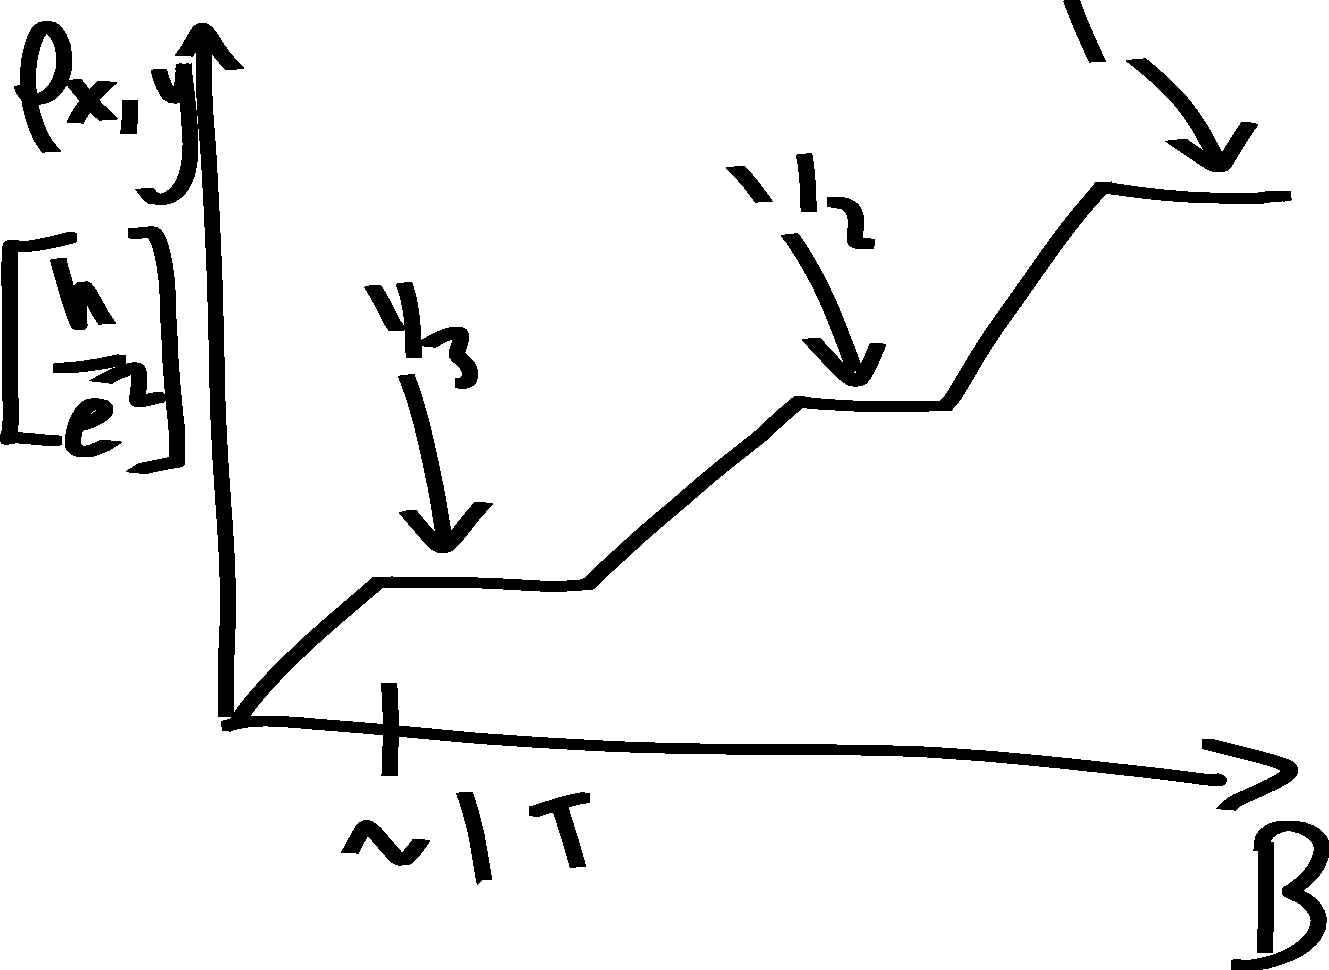
\includegraphics[width = 5in]{fig/quantum-hall-graph.pdf}
\end{center}
$\rho_{xx}$ on the other hand is roughly the same valueof $\rho_{xy}$, but it falls to zero at the plateaus.
This reflects an ``incompressible quantum state.''

This can be explained as follows: \me{(but note that I missed some parts of the following)} Suppose there's a single particle of charge $q$.
We get gapped states each with large degeneracy, via $\hbar \omega_B = q B/m$.
In particular, each particle takes fundamental flux $\phi_0 = 2 \pi \hbar / |e|$, so the total number of states at each energy is
\[
\frac{BA}{\phi_0}
\]
where $A$ is the area of the sample.
Idea is that each state has a ``bubble'' of flux around it and these don't overlap.
The plateaus happend because disorder/impurities spread out the degneracies.
The edges of these spreads are localized nonconductive states, so the first and last part of the increase in $B$ doesn't create any more conductivity.

The \emph{fractional} effect is more mysterious and more difficult to get.
It happens for fractions of the form $n/(2mn \pm 1)$.
It's mostly open why it happens.
One reason is that it depends heavily on the electron-electron interactions.
There are lots of these: if $\nu = 1/3$ then there are something like $\binom{N}{N/3}$ states, which is a \emph{lot.}

\subsection*{Connection to field theory}
Let $A = A_{\text{ext}}$ be the background EM field, with $\mathbf B = B \hat z$ and $\mathbf E = V_y \hat y$.
We write $\psi$ for the electrons in the sample.
Consider a partition function of the form
\[
\int e^{-\frac{i}{\hbar} S[A, \psi)]}.
\]
Here the effective action is
\[
S = \frac{k}{4 \pi} \int A \wedge dA
\]
This is topological, so how does it come from a condensed matter system?
It's reasonable if there are no propagating degrees of freedom.

We have
\[
\left \langle J_i(X) \right \rangle_A = \left \langle \frac{\delta S}{\delta A(x)} \right \rangle = \int \left( \frac{\delta S}{\delta A} e^{\frac{i}{\hbar} S}\right) \mathcal D \psi = \frac{\hbar}{i} \frac{\delta}{\delta A} \int e^{\frac{i}{\hbar} S} \mathcal D \psi = \frac{\delta}{\delta A} \left( e^{\frac{iS}{\hbar}} \right)
\]
so that
\[
\left \langle J_i \right \rangle =\frac{\delta S}{\delta A} = \frac{k}{2 \pi} \varepsilon_{ijk} F_{jk}
\]
Macroscopically, $J_i = k \varepsilon_{ij} E_j /2 \pi$, so $\sigma_{xy} = k/2 \pi$ and $\rho_{xy} = 2 \pi /k$ (where $\hbar = e = 1$.)

We now put the theory on a $2$-torus, so that
\[
S = \frac{k}{4 \pi} \int A \wedge dA = \frac{k}{4 \pi} \int (A_2 A_1 - A_1 A_2) \intd t \intd x \intd y = \frac{k}{2 \pi} \int A_2 \dot A_1 + \text{boundary terms} \intd t \intd x \intd y
\]\
and impose the gauge $A_0 = 0$.

There is one problem here: we still have a equation from varying $A_0$ that we'd now leave out, so we include it manually:
\[
0 = \frac{\delta S}{\delta A_0} = F_{12}.
\]
This means there's no field strength!

Furthermore, there are topological obstructions that can't be gauged away, namely the winding numbers
\[
\frac{1}{2 \pi} \oint_{C_i} A_i \intd x^i
\]
where $C_1, C_2$ are noncontractable loops around the torus.
%!TeX root = ../temp.tex
\section*{Lecture 15, 20/03/2018}
Today we discuss the BRST-BV formalism.
Recall that previously we worked with a BRST charge $Q$, $Q^2$, whose cohomology gives the physical states.
This can result in some complications (ghosts, ghosts for ghosts, etc.) but the point is to reduce the redundancy arising from gauge transformations.

We will now introduce new concepts: for each field there will be an antifield of opposite statistics and ghost number, which are necessary if the symmetry algebra is \emph{open.} (What that means will be discussed.)
There will also be an antibracket $(\,,\,)$ generalizing the Poisson bracket and pairing bosons and fermions, and a second-order operator $\Delta$.

Applications:
\begin{enumerate}
    \item Gauge theories where FP quantization doesn't work, like when the symmetry algebra is open:
    \[
    [\delta_\alpha, \delta_\beta] = f_{\alpha \beta}^\gamma(\phi) \delta_\gamma + \text{EoM}(\phi)
    \]
    This is complicated because the equations of motion know about the dynamics.
    \item Even in $3+1$ dimensional Yang-Mills it's hard to prove renormalizibility to all loop orders with just BRST.
    \item Lets you deal with anomalies in symmetries, both local and gauge.
    Has something to do with cohomology.
    For example, the chiral anomaly of the standard model is one-loop exact, and the proof doesn't really work unless you have BRST-BV. See Weinberg Chapter 22, Volume 2.
\end{enumerate}

What is an \emph{open} symmetry algebra?
Let's suppose we have an action
\[
S_0 = \int d^D x \mathcal{L}_0 (\phi^i, \partial_\mu \phi^i, \dots, \partial_{\mu_1} \cdots \partial_{\mu_k} \phi^i),
\]
which will then have equations of motion
\[
\frac{\delta \mathcal{L}_0}{\delta \phi^i(x)} = 0,
\]
which is to say
\[
\frac{\partial \mathcal{L}_0}{\partial \phi^i} - \partial_\mu \frac{\partial \mathcal{L}_0}{\partial (\partial_\mu\phi^i)} +  \partial_\mu  \partial_\nu \frac{\partial \mathcal{L}_0}{\partial (\partial_\mu \partial_\nu \phi^i)} - \cdots
\]
%!TeX root = ../temp.tex
\section*{Lecture 16, 22/03/2018}
Today: More about the BRST-BV formalism.
Recall that we made a choice of generating set $G$ of symmetries giving the Noether identities.
These can be written as
\[
\delta \phi^i = \lambda^\alpha(\phi) R_\alpha^i + M^{ij} \frac{\delta S_0}{\delta \phi^j}
\]
for some antisymmetric matrix $M^{ij}$.
Notice that here the $R_\alpha^i$ are in $G$.

The bracket of $R_\alpha^i$ and $R_\beta^j$ is a gauge transformation, so it must be expressible as
\[
R_\alpha^j \frac{\delta R_\beta^i}{\delta \phi^j} - R_\beta^j \frac{\delta R_\alpha^i}{\delta \phi^j} = C_{\alpha \beta}^{\phantom{\alpha \beta} \gamma}(\phi) R_\gamma^i + M_{\alpha \beta}^{ij}(f) \frac{\delta S_0}{\delta \phi^j}.
\]
The case where $M_{\alpha \beta}^ij$ is nonzero is when we get an open algebra of symmetries.
$G$ is \emph{reducible} if there are $\lambda^\alpha$ such that
\[
\lambda^\alpha R_\alpha^i = N^{ij} \frac{\delta S_0}{\delta \phi^j},
\]
for $N^{ij}$ antisymmetric, and \emph{irreducible} otherwise.

Example: Consider topological Yang-Mills, with symmetries $\delta A_\mu^a = \varepsilon_\mu^a(x) + D_\mu f^a(x)$.
The first (topological) terms gives ghosts $\psi_\mu^a(x)$, while the second (gauge) term gives $c^a(x)$.
These are redundant via $\varepsilon_\mu = -D_\mu f$.
We could try to eliminate them but this would not really be desirable.
\me{Maybe something to do with ghosts-for-ghosts?}

Recall that in Hamiltonian quantum mechanics with a phase space $\Phi$, observables are just $C^\infty(\Phi)$.
In QFT, Lorentz symmetry messes up the choice of time direction, so to generalize this approach we'll have to do something different.
One idea is to view a point $(p,q)$ as initial conditions for some solutions to the equations of motion.
If we have a nondegenerate Hamiltonian, there will be a one-to-one correspondence between such points and solutions of the equations of motion.
We therefore \emph{define} covariant phase space $\Sigma$ to be the set of all covariant solutions to the equations of motion.
(See Figure \ref{fig:phase-space}.)

\begin{figure}[h]
% \centering\includegraphics[width=2in]{fig.pdf}
\caption{A diagram of various phase-space reductions.}
\label{fig:phase-space}
\end{figure}

We can write $C^\infty(\Sigma) = C^\infty(\Phi)/\mathfrak{N}$, where $\mathfrak N$ is the ideal of functions vanishing on $\Sigma$.
We want to identify this as the cohomology $H^0(\delta)$ of some differential.
The easiest way to do this is by introducing an antifield $\phi_i^*$ for each field $\phi^i$ and declaring
\begin{align*}
\delta \phi^i &= 0\\
\delta \phi_i^* &= -\frac{\delta S_0}{\delta \phi^i}.
\end{align*}
(This is the Koszul-Tate construction.)
Notice that these antifields don't have anything to do with gauge symmetry.
We also introduce a quantum number \me{i.e.~grading} called the antighost number, which is $0$ for fields and $-1$ for antifields.
We will later identify this with minus the ghost number.

A reasonable question at this point is: What about $H^p(\delta)$ for $p > 0$?
It will create problems, but it occurs (also other times) when there is gauge symmetry: If we have a Noether identity
\[
\frac{\delta S_0}{\delta \phi^i} R_\alpha^i = 0,
\]
then
\[
\delta\left(R_\alpha^i \phi_i^* \right) = 0,
\]
but it isn't $\delta$ of anything, so we get a nontrivial class in $H^1(\delta)$.

To fix this problem, we can add a $\phi_\alpha^*$ with $\delta \phi_\alpha^* = R_\alpha^i \phi_i^*$.
Now there is a potential obstacle at ghost number $2$, and if there's more reducibility we might need to keep repeating this process, requiring more and more antifields.
This has something to do with derived categories/geometry.

It can be shown that for a generic gauge theory, $\Sigma$ splits nicely into gauge orbits: there's an integrability condition on the action of $G$.
In particular, we can assume that $\Sigma$ is a $G$-fibration over our desired gauge-invariant phase space $\Sigma/G$.
(Again, see Figure \ref{fig:phase-space}.)
This reduction is just BRST again!

Define \emph{vertical vectors} to be vectors on $\Sigma$ tangent to the $G$-orbits, and similarly for vertical $p$-forms.
Then we can define $d$ by (arguments vertical vectors)
\begin{align*}
dF(X) &= \frac{\delta}{\delta X}F\\
d \alpha(X,Y) = 0 - \mathcal{L}_Y \alpha(x) + \mathcal{L}_X \alpha(Y) + \alpha([X,Y]),
\end{align*}
and this will be the BRST charge.

Choose a basis of vertical vectors so that
\begin{align*}
X_\alpha F &= \frac{\delta F}{\delta \phi^i} R_\alpha^i\\
[X_\alpha, X_\beta] &= C_{\alpha \beta}^{\phantom{\alpha \beta} \gamma}(\phi) X_\gamma
\end{align*}
on $\Sigma$.
Introduce a basis $c^\alpha$ dual to $X_\alpha$, and define
\begin{align*}
dF &= (X_a F)c^\alpha\\
dc^\alpha &= \frac{1}{2} C_{\alpha \beta}^{\phantom{\alpha \beta} \gamma} c^\beta c^\gamma,
\end{align*}
which again is exactly the BRST charge action on the ghosts.

We now want to combine $\delta$ and $d$ together to a single operator $s$, but since $d \delta + \delta d \ne 0$, we can't just add them.
Instead we need to use \emph{homological perturbation theory}, which is a difficult piece of mathematics.
Once you know that it works, there's a shortcut:
Introduce an \emph{antibracket}
\[
sA = (A,S) 
\]
for a new object $S$.
We define $(\phi^i, \phi_j^*) = \delta^i_j$, $(c^\beta, \phi_\alpha^*) = \delta_\alpha^\beta$, etc.
The antibracket satisfies:
\begin{enumerate}
    \item $\operatorname{gh}\#(A,B) = \operatorname{gh}\# A + \operatorname{gh}\# B + 1$
    \item Parity $\epsilon(A,B)$ of $(A,B)$ is $\epsilon A + \epsilon B + 1$
    \item $(A,B) = (-1)^{(\epsilon A +1)(\epsilon B +1)}(B,A)$
    \item Super-Jacobi identity
\end{enumerate}
and if we choose $S$ so that $\operatorname{gh} \# S = 0$, $\epsilon S = 0$, $(S,S) =0$, then it will preserve the cohomology.
%!TeX root = ../main.tex
\section*{Guest Lecture 3a, 03/04/2018}
\me{I was absent.}
\section*{Guest Lecture 3b, 05/04/2018}
\me{I was absent.}
%!TeX root = ../main.tex
\section*{Lecture 17, 10/04/2018}
Today: The large-$N$ limit.
This has something to do with the AdS/CTF correspondence.
\me{Some historical discussion happened.}

Recall that in $SU(N)$ QCD there is no universally available expansion parameter, becasue the way renormalization works fixes a \emph{physical} scale $\Lambda_{QCD}$.
Therefore there is no universally available expansion parameter.
t'Hooft had the idea to deal with this by expanding in $1/N$, where $N$ is the rank of the gauge group.
It turns out that this can be made to work!
It's also relevant to statistical mechanics: H.E.~Stanley wrote a PRL paper (so it's short and readable) about trying to understand $O(n)$ spin models as $n \to \infty$.
Recall that $n = 0$ describes self-avoiding walks, $n =1$ is the Ising model, $n = 2$ is XY, and $n = 3$ is the Heisenberg model.

Similarly, t'Hooft has a paper on large $N$ QCD in $1+1$ dimensions, which someone presented in discussion.
We warm up with a simpler example, related to the $(1+1)$-dimensional Thirring model:
\[
S_T = \int d^2x \bar \psi i \slashed \partial \psi - g_T \bar (\psi \psi_\mu \psi)^2. 
\]
We previously sovled this model via bosonization.

Consider the similar Gross-Neveu model
\[
S_{GN} = \int d^2 x \bar \psi i \slashed d \psi - \frac{g}{2} (\bar \psi \psi)^2,
\]
where $\psi = \psi^a$, $a = 1, \dots , N$ is a Dirac spinor.
This model has a naive global $SU(N)$ symmetry; it can be extended to $SO(2N)$ by rotating particles and antiparticles into each other, but we don't need to do this.
Notice that for both theories the coupling constant is dimensionless.
This is a sort of baby QCD with only a matter sector.

This theory has a discrete chiral $\mathbb{Z}_2$ symmetry via $\psi \to - \gamma_3 \psi$, $\bar \psi \to - \bar \psi \gamma_3$.
There's no classical mass, but \me{something about asymptotic freedom.
I think that it will turn out to be so.}

In the $N \to \infty$ limit where there are no $1/N$ corrections, the propagator is just $\delta_{ab}$, and we can think about vertices splitting apart:
\[
\feynmandiagram[horizontal = a to b, baseline = (e.base)]{
    a [particle = $a$] --[fermion] e --[fermion] b [particle = $a$],
    c [particle = $b$] --[fermion] e --[fermion] d [particle = $b$]
};
=
\feynmandiagram[vertical = e1 to e2, baseline = (e1.base)]{
    a [particle = $a$] --[fermion] e1 --[fermion] b [particle = $a$],
    c [particle = $b$] --[fermion] e2 --[fermion] d [particle = $b$],
    e1 -- [ghost] e2
};
\]
Now the expansion of an $a, \bar a \to b , \bar b$ scattering looks like
\begin{center}
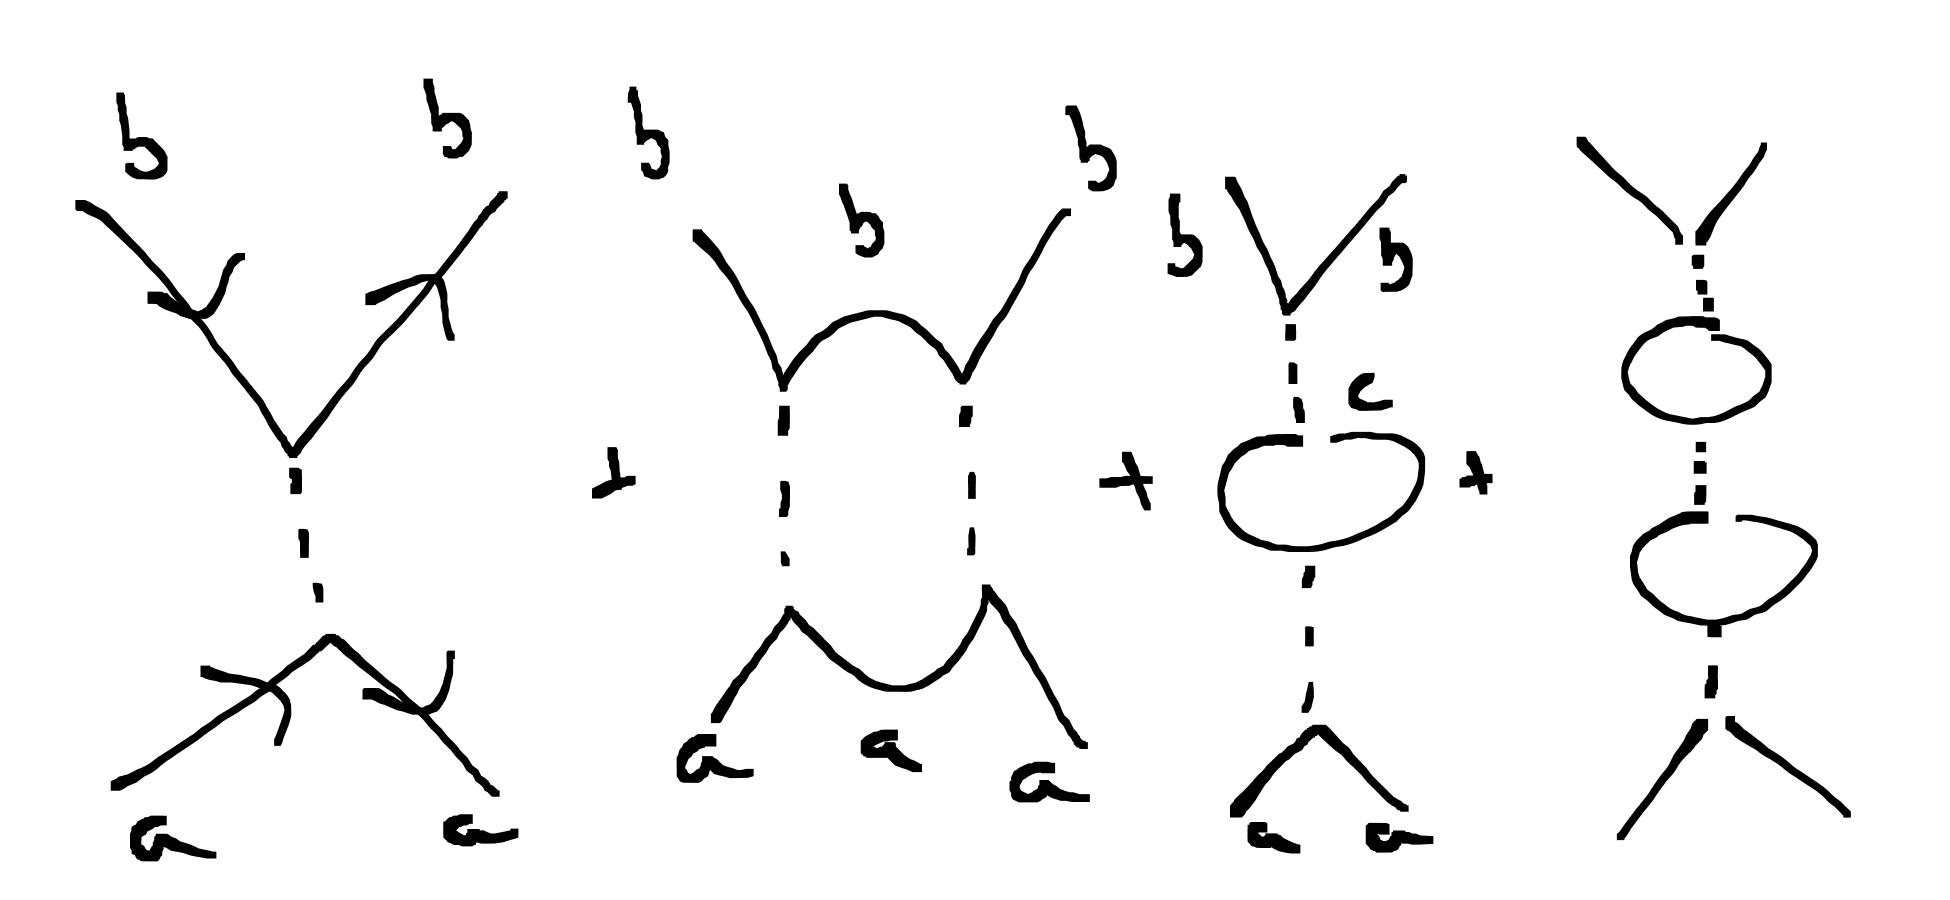
\includegraphics{fig/largeNexample.png}
\end{center}
\me{This \emph{could} be done in tikzFeynman but would probably require manual vertex placement.
I did not feel like dealing with that.}
Note that these are just representative terms.
When you take the traces in the loops these terms are order $g$, $g^2$, $g^2 n$, and $g^3 N^2$ respectively.
This will not work as $N \to \infty$.
We need a new coupling $\lambda^2 = gN$, which is fixed as $N \to \infty$.
The expansion terms above are now $\lambda^2/N$, $\lambda^4/N^2$, $\lambda^4/N$, $\lambda^6/N$, so they can converge.

We can then rewrite the action as
\[
\int d^2 x \bar \psi i \slashed \partial \psi - \frac{\lambda^2}{2 N}(\bar \psi \psi)^2.
\]
You might think that this will be free in the $N \to \infty$ limit, but this doesn't quite work, because there's an $N$ in the first term.

To deal with this question, introduce an auxiliary field
\[
\sigma = \frac{\lambda}{N} \bar \psi \psi.
\]
We can now integrate out $\bar \psi$ and $\psi$ to get an effective potential
\[
-i V(\sigma_0) = - i \frac{N}{2 \lambda^2} \sigma^2 - N \sum_{r=1}^\infty \frac{1}{2r} \tr \int \frac{d^2 p}{(2 \pi)^2} \left(\frac{- \slashed p \sigma}{p^3} \right)^{2r},
\]
so that
\[
V = \frac{N}{2 \lambda^2} \sigma - N \int \frac{d^2 p}{(2 \pi)^2} \log\left( 1 + \frac{\sigma_0}{\me{??}} \right).
\]
This gives an effective mass for $\psi$ and breaks the chiral symmetry.

\me{I missed a portion of the following discussion.}
$\sigma$ is a \emph{master field.}
It is possible to associate $1/N \sim \hbar$ and get a classical limit.

\subsection*{More systematic approach to large $N$}
Consider a generic QFT of some fields $M$, which we take to be matrices in some simple Lie group, say $U(N)$.
\me{There was a comment about choosing them Hermitian, which would mean that they're in the Lie algebra.
Since this is field theory, those are the same thing.}
The action is of the form
\[
S = \int \tr \left[ (\partial M)^2 + \highlight{M^2 + M^3 + \cdots} \right]
\]
with the \highlight{highlighted terms} grouped together to give a potential $V(M)$.
Because the matrices have \emph{two} indices, the propagators have two edges and the Feynman diagrams are \emph{ribbon} graphs.

Notice that the propagators contribute $g^2$, the vertices contribute $1/g^2$, and the loops contribute an $N$ from the trace.
Therefore a general diagram scales as
\[
(g^2)^{P - V} N^L = (g^2 N)^{P - V} N^{V - P + L}
\]
where $P$ is the number of propagators (edges), $V$ the number of vertices, and $L$ the number of loops.
The second term above is $(1/N)^{2g -2}$, where $g$ is the genus of the ribbon graph.
This is one way to motivate string theory: we have a perturbative expansion over surfaces.
%!TeX root = ../main.tex
\section*{Lecture 18, 12/04/2018}
Review of last time.
\me{There was a discussion of the topology of surfaces and of various ways to compute the Euler characteristic.}

Recall that using the new coupling constant $\lambda = gN^2$, the order of each diagram is
\[
\lambda^{P-V} N^{V-P+L} = \lambda^{P-V}N^\chi
\]
where $P$ is the number of propagators/edges, $V$ is the number of vertices, $L$ is the number of loops, and $\chi$ is the Euler characteristic of the surface associated to the ribbon graph diagram.
The partition function is then
\[
\mathcal Z = \sum_{g =0}^\infty \left( \frac{1}{N} \right)^{2g-2} \sum_{\text{diagrams of genus } g} f(\lambda)
\]
for some functions $f$ depending only on the coupling $\lambda$.
This type of formula will hold for \emph{any} quantum theory of matrices.
\me{I think this may just be a statement about sums over ribbon graphs.}

This gives a connection to string theory, where our provisional definition of a string theory is something where the Feynman diagrams are ribbon graphs.
In order to interpret the above sum, we'd like to view it as one.
Unfortunately, very few string theories are known; basically the only one is superstring theory in 10 dimensions.
That has a bunch of supersymmetries, so where do they show up in the large $N$ theory?

More generally, general QFTs are hard, so it may be overly ambitious to try this with them.
Instead we look at CFTs.
\me{There was a discussion of fixed points of the RG flow that I didn't follow.}
This will turn out to work because there's a connection to supersymmetry.
Both theories are representations of $SO(4,2)$, the symmetries of $\mathbb{R}^{3,1}$.
How does it act on the string theory side?

We postulate that the genus-$g$ contribution to the partition function is of the form
\[
F_g(\lambda) = \int \mathcal D (\text{fields}) e^{i S}
\]
where $S$ is an integral of the fields over the ``string worldsheet,'' which is just a surface $\Sigma$ of genus $g$.
We could have a ``cartoon'' Polyakov action
\[
 S = d^2 \sigma \partial_\alpha x^\mu \partial_\alpha x^\nu \eta_{\mu \nu},
\]
where $\sigma$ is the worldsheet coordinate indexed by $\alpha$ and $\mu$ is the spacetime coordinate; the fields are just a map $x^\mu : \Sigma \to M$ for $M$ a $4$-manifold.

This manifold isn't high-dimensional enough to have isometry group $SO(4,2)$, so we pass to a new spacetime $\hat M$ by adding a dimension $u$.
The metric will then be
\[
ds^2 = w(u)^2 \left( dx^\mu dx^\nu \eta_{\mu \nu} + du^2 \right),
\]
where $w(u)$ is the \emph{warp factor.}
To get conformal symmetry, we then have to set $w^2 = 1/u^2$.
But we now have anti-de Sitter space in $4+1$ dimensions, in Poincar\'e patch coordinates.
Recall that anti-de Sitter space is the maximally symmetric solution to the Einstein equations with negative cosmological constant.

$SO(4,2)$ has 32 generators (supercharges) which we can think of as corresponding to four Majorana fermions.
They can be rotated into each other, so we get additional bosonic symmetries in the form of an $SU(4)$ factor.
This corresponds with taking the product of $\hat M$ with $S^5$.

We have seen that there's a connection between a large $N$ theory of matrices and string theory.
We will later see that if the matrix theory has a local energy-momentum tensor, the string theory will have a gravity-like excitation.
\me{There was as further discussion of the relationship between the conformal dimension of the CFT and the mass in the AdS side but I did not follow the details.}
%!TeX root = ../main.tex
\section*{Lecture 19, 17/04/2018}
Today: more on large $N$ and AdS/CFT

To get CFT out of large $N$, we add conformal symmetry and therefore look for RG fixed points.
In $3+1$ dimensions we need symmetry group $SO(4,2)$, which then forces spacetime to be $5$-dimensional.
The resulting metric is 
\[
ds^2 = L^2 \left( \frac{d \vc x d \vc x}{u^2} = \frac{du^2}{u^2}\right).
\]
One reason this is reasonable is that this spacetime should be foliated by regular spacetime in the $u$ direction.
Radial evolution in this anti-de Sitter spacetime should correspond to the RG flow.
Here $L$ is the radius.

There is also a ``UV-IR'' duality, in that the UV limit of the CFT corresponds to the IR limit of gravity.

Another question is how to deal with this correspondence globally in AdS space, instead of just the part with our particular coordinate system.
The boundary of the whole spacetime is $S^3 \times \mathbb{R}$, whose metric is determined only up to conformal scalings.
We will not discuss this much.

To see that the AdS theory actually has gravity:
Consider the partition function
\[
 \mathcal Z_{\text{bulk}} \left [\left . \phi(\vc x, u) \right |_{u = 0 \text{ on } \partial \hat{\mathcal M}} = \phi_0 (\vc x) \right ] = \left \langle \exp \int d^4x\, \phi_0(\vc x) \mathcal O(\vc x) \right \rangle,
\]
where we have identified the boundary values of the bulk fields with the source term.

For example: consider a scalar field $\phi$ of mass $m$ in the bulk.
Then
\[
S = \frac{1}{2} \int d^4x \, du \, \sqrt{-G} G^{MN} \partial_M \phi \partial_N \phi - \frac{1}{2} m^2 \phi^2,
\]
where $G^{MN}$ is the AdS metric from before.
The classical equations of motion are more complicated because spacetime is no longer flat.
Near $u = 0$, we assume $\phi \sim u^\alpha$ for large $\phi$.
We can then check that
\[
\alpha (\alpha -4) - m^2 L^2 = 0,
\]
so there are two solutions $\alpha_\pm = 2 \pm \sqrt{4 + m^2 L^2}$.
$\alpha_-$ always dominates near the boundary, and $\alpha_+$ always decays.
We thus get $m^2 L^2 \ge 4$, the Breitenlohner-Freedman bound.
Claim: For $\phi$, the associated operator $\mathcal O$ has conformal dimension $\Delta = 2 + \sqrt{4 + m^2 L^2}$.

The expectation value is UV divergent, which corresponds to an IR divergence in the bulk partition function in the AdS side.
We can fix this divergence by dcurring things off close to the boundary, in which case
\[
\phi(\vc x, u)|_{u = \varepsilon} = \varepsilon^\alpha - \phi_0^R(\vc x),
\]
and we can extract $\phi_0^R$ as the renormalized field.

What are the scaling dimensions under the scaling $\vc x \to \lambda \vc x$, $u \to \lambda u$?
We can compute $[\phi^R] = \alpha_-$, $[\mathcal O] = 4 - \alpha_- = \alpha_+$.
At $m = 0$ we get $[\mathcal O] = 4$.
How many interesting dimension 4 CFT operators do we know?
\me{Something to do with 4 dimensional SUSY Yang-Mills.}
In particular there is a massless dilaton-like field in the bulk.

Recall that the scaling dimension of $T^{\mu \nu}$ is $4$, so this should correspond to a mass-zero spin-2 field in the bulk, i.e.~a graviton.

In the limit of classical gravity,
\[
W_{\text{eff}} = S_{\text{on-shell}}[\phi_0^R]_{\text{gravity}}.
\]
The on-shell part is
\[
S_{\text{on-shell}} = \frac{1}{16 \pi G_n} \int d^4x\, \sqrt{-g} \mathcal L
\]
where we take only the IR-regular or $\log \varepsilon$ part of the Lagrangian.

\me{At this point my physics knowledge started to become lacking and my notes were no longer useful.}
%!TeX root = ../main.tex
\section*{Lectures 20-22}
\me{For various reasons I was not at these lectures, so I didn't take notes.}
\end{document}